% Copyright (c) 2025 Alexander Bluhm <bluhm@genua.de>
%
% Permission to use, copy, modify, and distribute this software for any
% purpose with or without fee is hereby granted, provided that the above
% copyright notice and this permission notice appear in all copies.
%
% THE SOFTWARE IS PROVIDED "AS IS" AND THE AUTHOR DISCLAIMS ALL WARRANTIES
% WITH REGARD TO THIS SOFTWARE INCLUDING ALL IMPLIED WARRANTIES OF
% MERCHANTABILITY AND FITNESS. IN NO EVENT SHALL THE AUTHOR BE LIABLE FOR
% ANY SPECIAL, DIRECT, INDIRECT, OR CONSEQUENTIAL DAMAGES OR ANY DAMAGES
% WHATSOEVER RESULTING FROM LOSS OF USE, DATA OR PROFITS, WHETHER IN AN
% ACTION OF CONTRACT, NEGLIGENCE OR OTHER TORTIOUS ACTION, ARISING OUT OF
% OR IN CONNECTION WITH THE USE OR PERFORMANCE OF THIS SOFTWARE.

\documentclass[14pt,aspectratio=169]{beamer}
\usetheme{Frankfurt}
\usepackage{tikz}
\usepackage{framed}
\usepackage{adjustbox}
\usepackage{graphicx}
\usepackage{grffile}
\usepackage{varwidth}
\usepackage{tipa}
\usepackage{alltt}
\usepackage{xcolor}
\usepackage{upquote}
\usepackage[T1]{fontenc}
\usepackage{textcomp}
\usepackage{calc}
\usetikzlibrary{shapes.arrows}
\usetikzlibrary{shapes.geometric}
\usetikzlibrary{shapes.multipart}
\usetikzlibrary{shapes.symbols}

\author{Alexander Bluhm}
\title{Update on OpenBSD Networking Performance Improvements}
\institute{bluhm@openbsd.org}
\date{EuroBSDCon, September 2025}

\begin{document}

\begin{frame}
\titlepage
\end{frame}

\begin{frame}{Agenda}
\setcounter{tocdepth}{1}
\tableofcontents
\end{frame}

\section{History}

\subsection{Single Processor SPL}
\begin{frame}{Single Processor SPL, 1980s}
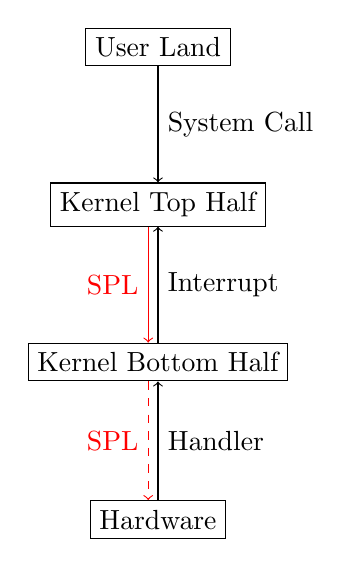
\begin{tikzpicture}
    \path (0, 0) node [draw] (ul) {User Land};
    \path (0, -2) node [draw] (to) {Kernel Top Half};
    \draw [->] (ul) -- (to) node[midway,right] {System Call};
    \path (0, -4) node [draw] (bo) {Kernel Bottom Half};
    \draw [<-] (to.south) -- (bo.north) node[midway,right] {Interrupt};
    \path (to.south) node (tos) {} (bo.north) node (bon) {};
    \draw [->,red] (tos.west) -- (bon.west) node[midway,left,red] {SPL};
    \path (0, -6) node [draw] (hw) {Hardware};
    \draw [<-] (bo) -- (hw) node[midway,right] {Handler};
    \path (bo.south) node (bos) {} (hw.north) node (hwn) {};
    \draw [->,red,dashed] (bos.west) -- (hwn.west) node[midway,left,red] {SPL};
\end{tikzpicture}
\end{frame}

\subsection{Softnet AST}
\begin{frame}{Softnet AST, 1990s}
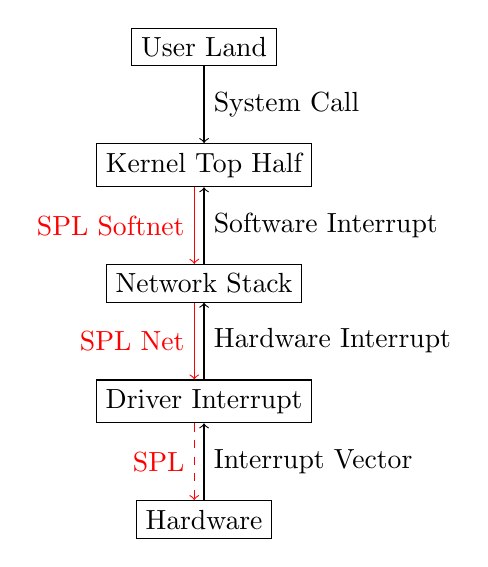
\begin{tikzpicture}
    \path (0, 0) node [draw] (ul) {User Land};
    \path (0, -1.5) node [draw] (to) {Kernel Top Half};
    \draw [->] (ul) -- (to) node[midway,right] {System Call};
    \path (0, -3) node [draw] (ns) {Network Stack};
    \draw [<-] (to.south) -- (ns.north) node[midway,right] {Software Interrupt};
    \path (to.south) node (tos) {} (ns.north) node (nsn) {};
    \draw [->,red] (tos.west) -- (nsn.west) node[midway,left,red] {SPL Softnet};
    \path (0, -4.5) node [draw] (di) {Driver Interrupt};
    \draw [<-] (ns.south) -- (di.north) node[midway,right] {Hardware Interrupt};
    \path (ns.south) node (nss) {} (di.north) node (din) {};
    \draw [->,red] (nss.west) -- (din.west) node[midway,left,red] {SPL Net};
    \path (0, -6) node [draw] (hw) {Hardware};
    \draw [<-] (di) -- (hw) node[midway,right] {Interrupt Vector};
    \path (di.south) node (dis) {} (hw.north) node (hwn) {};
    \draw [->,red,dashed] (dis.west) -- (hwn.west) node[midway,left,red] {SPL};
\end{tikzpicture}
\end{frame}

\subsection{Multi Processor Kernel Lock}
\begin{frame}{Multi Processor Kernel Lock, 2000s}
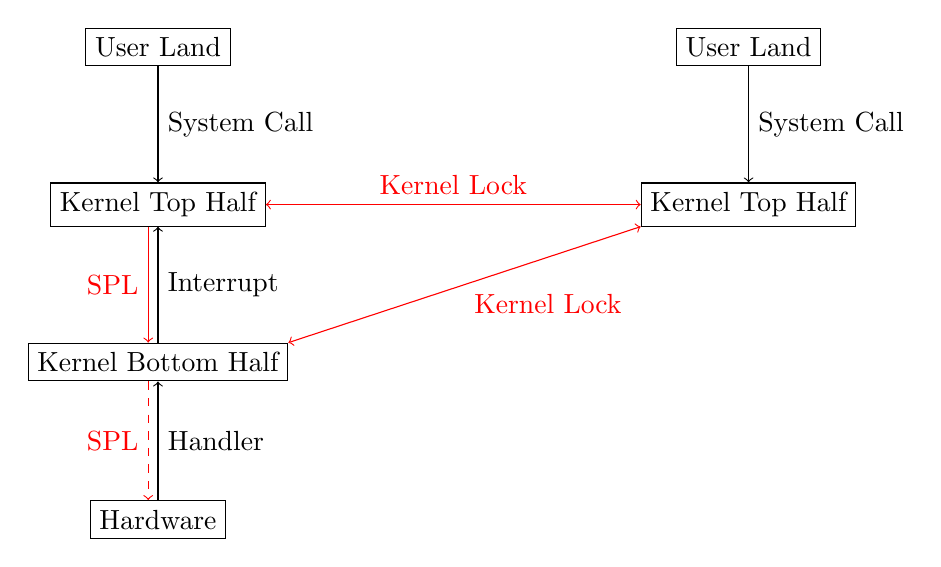
\begin{tikzpicture}
    \path (0, 0) node [draw] (ul) {User Land};
    \path (0, -2) node [draw] (to) {Kernel Top Half};
    \draw [->] (ul) -- (to) node[midway,right] {System Call};
    \path (0, -4) node [draw] (bo) {Kernel Bottom Half};
    \draw [<-] (to.south) -- (bo.north) node[midway,right] {Interrupt};
    \path (to.south) node (tos) {} (bo.north) node (bon) {};
    \draw [->,red] (tos.west) -- (bon.west) node[midway,left,red] {SPL};
    \path (0, -6) node [draw] (hw) {Hardware};
    \draw [<-] (bo) -- (hw) node[midway,right] {Handler};
    \path (bo.south) node (bos) {} (hw.north) node (hwn) {};
    \draw [->,red,dashed] (bos.west) -- (hwn.west) node[midway,left,red] {SPL};

    \path (7.5, 0) node [draw] (ul1) {User Land};
    \path (7.5, -2) node [draw] (to1) {Kernel Top Half};
    \draw [->] (ul1) -- (to1) node[midway,right] {System Call};

    \draw [<->,red] (to) -- (to1) node[midway,above] {Kernel Lock};
    \draw [<->,red] (bo.north east) -- (to1.south west)
	node[midway,below right] {Kernel Lock};
\end{tikzpicture}
\end{frame}

\subsection{Kernel Lock and Network Lock}
\begin{frame}{Kernel Lock and Net Lock, 2015}
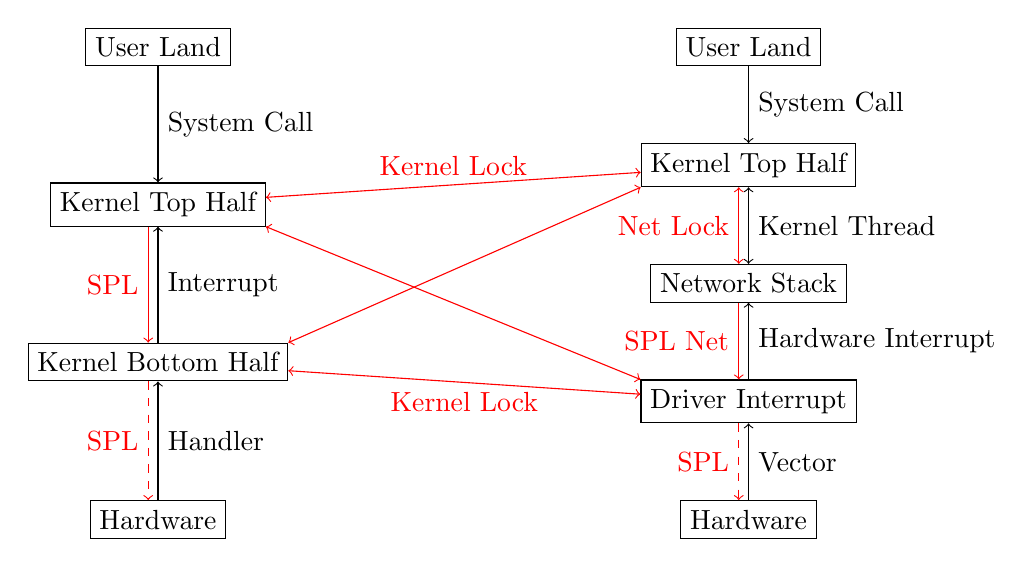
\begin{tikzpicture}
    \path (0, 0) node [draw] (ul) {User Land};
    \path (0, -2) node [draw] (to) {Kernel Top Half};
    \draw [->] (ul) -- (to) node[midway,right] {System Call};
    \path (0, -4) node [draw] (bo) {Kernel Bottom Half};
    \draw [<-] (to.south) -- (bo.north) node[midway,right] {Interrupt};
    \path (to.south) node (tos) {} (bo.north) node (bon) {};
    \draw [->,red] (tos.west) -- (bon.west) node[midway,left,red] {SPL};
    \path (0, -6) node [draw] (hw) {Hardware};
    \draw [<-] (bo) -- (hw) node[midway,right] {Handler};
    \path (bo.south) node (bos) {} (hw.north) node (hwn) {};
    \draw [->,red,dashed] (bos.west) -- (hwn.west) node[midway,left,red]
	{SPL};

    \path (7.5, 0) node [draw] (ul1) {User Land};
    \path (7.5, -1.5) node [draw] (to1) {Kernel Top Half};
    \draw [->] (ul1) -- (to1) node[midway,right] {System Call};
    \path (7.5, -3) node [draw] (ns1) {Network Stack};
    \draw [<->] (to1.south) -- (ns1.north) node[midway,right] {Kernel Thread};
    \path (to1.south) node (tos1) {} (ns1.north) node (nsn1) {};
    \draw [<->,red] (tos1.west) -- (nsn1.west) node[midway,left,red] {Net Lock};
    \path (7.5, -4.5) node [draw] (di1) {Driver Interrupt};
    \draw [<-] (ns1.south) -- (di1.north) node[midway,right]
	{Hardware Interrupt};
    \path (ns1.south) node (nss1) {} (di1.north) node (din1) {};
    \draw [->,red] (nss1.west) -- (din1.west) node[midway,left,red] {SPL Net};
    \path (7.5, -6) node [draw] (hw1) {Hardware};
    \draw [<-] (di1) -- (hw1) node[midway,right] {Vector};
    \path (di1.south) node (dis1) {} (hw1.north) node (hwn1) {};
    \draw [->,red,dashed] (dis1.west) -- (hwn1.west) node[midway,left,red]
	{SPL};

    \draw [<->,red] (to) -- (to1) node[midway,above] {Kernel Lock};
    \draw [<->,red] (bo.north east) -- (to1.south west);
    \draw [<->,red] (to.south east) -- (di1.north west);
    \draw [<->,red] (bo) -- (di1) node[midway,below] {Kernel Lock};
\end{tikzpicture}
\end{frame}

\subsection{Unlock Network System Calls}
\begin{frame}{Unlock Network System Calls, 2018}
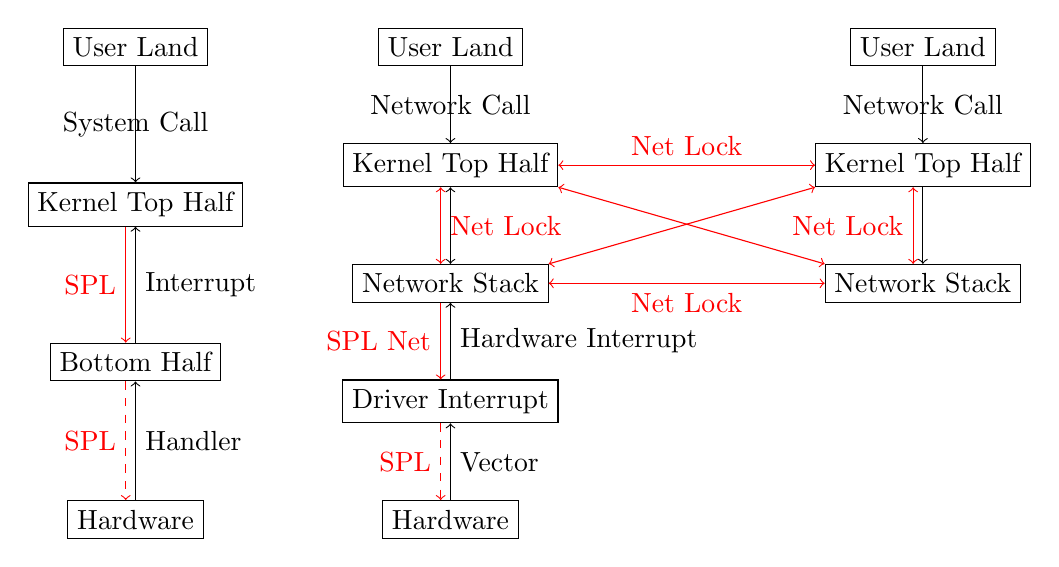
\begin{tikzpicture}
    \path (0, 0) node [draw] (ul) {User Land};
    \path (0, -2) node [draw] (to) {Kernel Top Half};
    \draw [->] (ul) -- (to) node[midway] {System Call};
    \path (0, -4) node [draw] (bo) {Bottom Half};
    \draw [<-] (to.south) -- (bo.north) node[midway,right] {Interrupt};
    \path (to.south) node (tos) {} (bo.north) node (bon) {};
    \draw [->,red] (tos.west) -- (bon.west) node[midway,left,red] {SPL};
    \path (0, -6) node [draw] (hw) {Hardware};
    \draw [<-] (bo) -- (hw) node[midway,right] {Handler};
    \path (bo.south) node (bos) {} (hw.north) node (hwn) {};
    \draw [->,red,dashed] (bos.west) -- (hwn.west) node[midway,left,red]
	{SPL};

    \path (4, 0) node [draw] (ul1) {User Land};
    \path (4, -1.5) node [draw] (to1) {Kernel Top Half};
    \draw [->] (ul1) -- (to1) node[midway] {Network Call};
    \path (4, -3) node [draw] (ns1) {Network Stack};
    \draw [<->] (to1.south) -- (ns1.north) node[midway,right] {};
    \path (to1.south) node (tos1) {} (ns1.north) node (nsn1) {};
    \draw [<->,red] (tos1.west) -- (nsn1.west) node[midway,right,red]
	{Net Lock};
    \path (4, -4.5) node [draw] (di1) {Driver Interrupt};
    \draw [<-] (ns1.south) -- (di1.north) node[midway,right]
	{Hardware Interrupt};
    \path (ns1.south) node (nss1) {} (di1.north) node (din1) {};
    \draw [->,red] (nss1.west) -- (din1.west) node[midway,left,red] {SPL Net};
    \path (4, -6) node [draw] (hw1) {Hardware};
    \draw [<-] (di1) -- (hw1) node[midway,right] {Vector};
    \path (di1.south) node (dis1) {} (hw1.north) node (hwn1) {};
    \draw [->,red,dashed] (dis1.west) -- (hwn1.west) node[midway,left,red]
	{SPL};

    \path (10, 0) node [draw] (ul2) {User Land};
    \path (10, -1.5) node [draw] (to2) {Kernel Top Half};
    \draw [->] (ul2) -- (to2) node[midway] {Network Call};
    \path (10, -3) node [draw] (ns2) {Network Stack};
    \draw [->] (to2.south) -- (ns2.north) node[midway,right] {};
    \path (to2.south) node (tos2) {} (ns2.north) node (nsn2) {};
    \draw [<->,red] (tos2.west) -- (nsn2.west) node[midway,left,red] {Net Lock};

    \draw [<->,red] (to1) -- (to2) node[midway,above] {Net Lock};
    \draw [<->,red] (ns1.north east) -- (to2.south west);
    \draw [<->,red] (to1.south east) -- (ns2.north west);
    \draw [<->,red] (ns1) -- (ns2) node[midway,below] {Net Lock};
\end{tikzpicture}
\end{frame}

\subsection{Multi Queue Drivers}
\begin{frame}{Multi Queue Drivers, 2020}
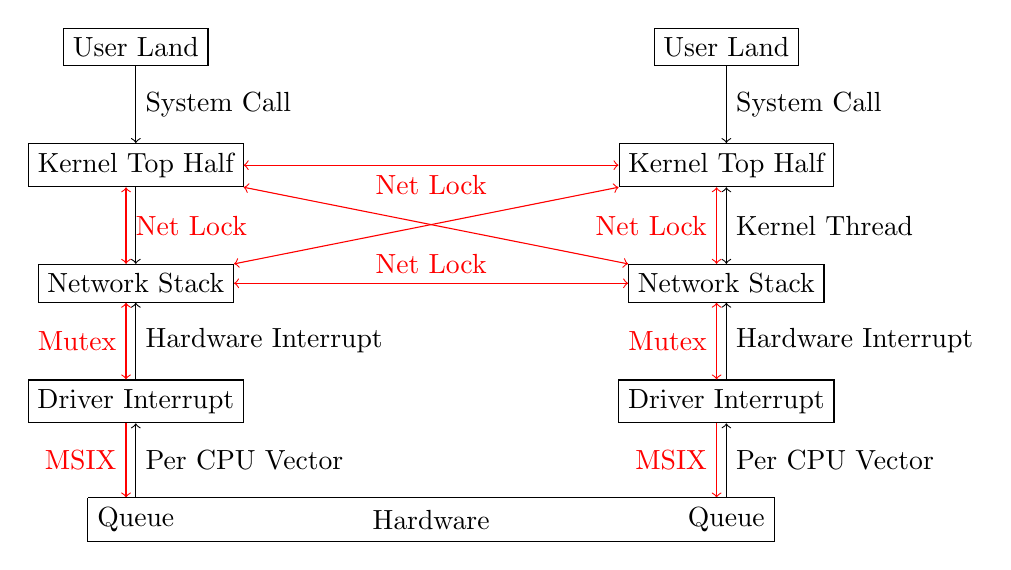
\begin{tikzpicture}
    \path (0, 0) node [draw] (ul) {User Land};
    \path (0, -1.5) node [draw] (to) {Kernel Top Half};
    \draw [->] (ul) -- (to) node[midway,right] {System Call};
    \path (0, -3) node [draw] (ns) {Network Stack};
    \draw [->] (to.south) -- (ns.north) node[midway,right] {};
    \path (to.south) node (tos) {} (ns.north) node (nsn) {};
    \draw [<->,red] (tos.west) -- (nsn.west) node[midway,right,red] {Net Lock};
    \path (0, -4.5) node [draw] (di) {Driver Interrupt};
    \draw [<-] (ns.south) -- (di.north) node[midway,right]
	{Hardware Interrupt};
    \path (ns.south) node (nss) {} (di.north) node (din) {};
    \draw [<->,red] (nss.west) -- (din.west) node[midway,left,red] {Mutex};
    \path (0, -6) node (hw) {Queue};
    \draw [<-] (di) -- (hw) node[midway,right] {Per CPU Vector};
    \path (di.south) node (dis) {} (hw.north) node (hwn) {};
    \draw [->,red] (dis.west) -- (hwn.west) node[midway,left,red] {MSIX};

    \path (7.5, 0) node [draw] (ul1) {User Land};
    \path (7.5, -1.5) node [draw] (to1) {Kernel Top Half};
    \draw [->] (ul1) -- (to1) node[midway,right] {System Call};
    \path (7.5, -3) node [draw] (ns1) {Network Stack};
    \draw [<->] (to1.south) -- (ns1.north) node[midway,right] {Kernel Thread};
    \path (to1.south) node (tos1) {} (ns1.north) node (nsn1) {};
    \draw [<->,red] (tos1.west) -- (nsn1.west) node[midway,left,red] {Net Lock};
    \path (7.5, -4.5) node [draw] (di1) {Driver Interrupt};
    \draw [<-] (ns1.south) -- (di1.north) node[midway,right]
	{Hardware Interrupt};
    \path (ns1.south) node (nss1) {} (di1.north) node (din1) {};
    \draw [<->,red] (nss1.west) -- (din1.west) node[midway,left,red] {Mutex};
    \path (7.5, -6) node (hw1) {Queue};
    \draw [<-] (di1) -- (hw1) node[midway,right] {Per CPU Vector};
    \path (di1.south) node (dis1) {} (hw1.north) node (hwn1) {};
    \draw [->,red] (dis1.west) -- (hwn1.west) node[midway,left,red] {MSIX};

    \draw [<->,red] (to) -- (to1) node[midway,below] {Net Lock};
    \draw [<->,red] (ns.north east) -- (to1.south west) node[midway] {};
    \draw [<->,red] (to.south east) -- (ns1.north west) node[midway] {};
    \draw [<->,red] (ns) -- (ns1) node[midway,above] {Net Lock};
    \draw [-] (hw.north west) -- (hw1.north east) -- (hw1.south east) --
	(hw.south west) -- (hw.north west);
    \path (hw) -- (hw1) node[midway] {Hardware};
\end{tikzpicture}
\end{frame}

\subsection{Unlock Socket Receive Send}
\begin{frame}{Unlock Socket Receive and Send, 2022 and 2024}
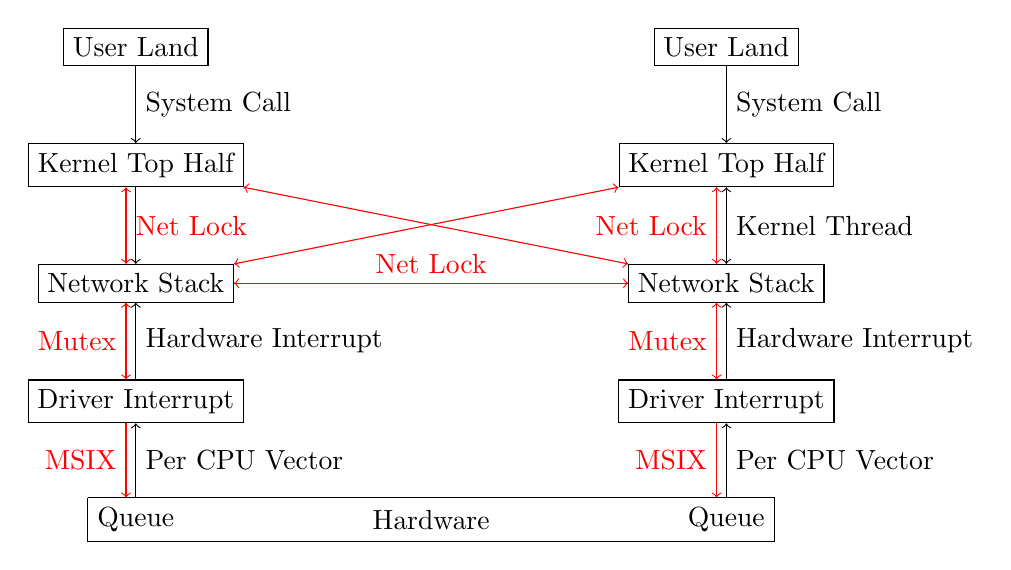
\begin{tikzpicture}
    \path (0, 0) node [draw] (ul) {User Land};
    \path (0, -1.5) node [draw] (to) {Kernel Top Half};
    \draw [->] (ul) -- (to) node[midway,right] {System Call};
    \path (0, -3) node [draw] (ns) {Network Stack};
    \draw [->] (to.south) -- (ns.north) node[midway,right] {};
    \path (to.south) node (tos) {} (ns.north) node (nsn) {};
    \draw [<->,red] (tos.west) -- (nsn.west) node[midway,right,red] {Net Lock};
    \path (0, -4.5) node [draw] (di) {Driver Interrupt};
    \draw [<-] (ns.south) -- (di.north) node[midway,right]
	{Hardware Interrupt};
    \path (ns.south) node (nss) {} (di.north) node (din) {};
    \draw [<->,red] (nss.west) -- (din.west) node[midway,left,red] {Mutex};
    \path (0, -6) node (hw) {Queue};
    \draw [<-] (di) -- (hw) node[midway,right] {Per CPU Vector};
    \path (di.south) node (dis) {} (hw.north) node (hwn) {};
    \draw [->,red] (dis.west) -- (hwn.west) node[midway,left,red] {MSIX};

    \path (7.5, 0) node [draw] (ul1) {User Land};
    \path (7.5, -1.5) node [draw] (to1) {Kernel Top Half};
    \draw [->] (ul1) -- (to1) node[midway,right] {System Call};
    \path (7.5, -3) node [draw] (ns1) {Network Stack};
    \draw [<->] (to1.south) -- (ns1.north) node[midway,right] {Kernel Thread};
    \path (to1.south) node (tos1) {} (ns1.north) node (nsn1) {};
    \draw [<->,red] (tos1.west) -- (nsn1.west) node[midway,left,red] {Net Lock};
    \path (7.5, -4.5) node [draw] (di1) {Driver Interrupt};
    \draw [<-] (ns1.south) -- (di1.north) node[midway,right]
	{Hardware Interrupt};
    \path (ns1.south) node (nss1) {} (di1.north) node (din1) {};
    \draw [<->,red] (nss1.west) -- (din1.west) node[midway,left,red] {Mutex};
    \path (7.5, -6) node (hw1) {Queue};
    \draw [<-] (di1) -- (hw1) node[midway,right] {Per CPU Vector};
    \path (di1.south) node (dis1) {} (hw1.north) node (hwn1) {};
    \draw [->,red] (dis1.west) -- (hwn1.west) node[midway,left,red] {MSIX};

    \draw [<->,red] (ns.north east) -- (to1.south west) node[midway] {};
    \draw [<->,red] (to.south east) -- (ns1.north west) node[midway] {};
    \draw [<->,red] (ns) -- (ns1) node[midway,above] {Net Lock};
    \draw [-] (hw.north west) -- (hw1.north east) -- (hw1.south east) --
	(hw.south west) -- (hw.north west);
    \path (hw) -- (hw1) node[midway] {Hardware};
\end{tikzpicture}
\end{frame}

\subsection{Parallel Forwarding}
\begin{frame}{Parallel Forwarding, 2022}
\begin{tikzpicture}
    \path (0, -.5) node (ul) {};
    \path (0, -1.5) node [draw] (so) {Socket Layer};
    \draw [->] (ul) -- (so) node[near start,right] {Receive};
    \path (0, -3) node [draw] (pr) {TCP/UDP Protocol};
    \draw [<-] (so.south) -- (pr.north) node[midway,right] {};
    \path (so.south) node (sos) {} (pr.north) node (prn) {};
    \draw [<->,red] (sos.west) -- (prn.west) node[midway,right,red] {Net Lock};
    \path (0, -4.5) node [draw] (ip) {IP Stack};
    \draw [<-] (pr.south) -- (ip.north) node[midway,right] {Net Queue};
    \path (0, -6) node [draw] (dr) {Driver};
    \draw [<-] (ip) -- (dr) node[midway,right] {Interrupt};
    \path (0, -7.0) node  (hw) {};
    \draw [<-] (dr) -- (hw) node[near end,right] {Per CPU};

    \path (7.5, -.5) node (ul1) {};
    \path (7.5, -1.5) node [draw] (so1) {Socket Layer};
    \draw [->] (ul1) -- (so1) node[near start,right] {Send};
    \path (7.5, -3) node [draw] (pr1) {TCP/UDP Protocol};
    \draw [->] (to1.south) -- (pr1.north) node[midway,right] {};
    \path (so1.south) node (sos1) {} (pr1.north) node (prn1) {};
    \draw [<->,red] (sos1.west) -- (prn1.west) node[midway,left,red] {Net Lock};
    \path (7.5, -4.5) node [draw] (ip1) {IP Stack};
    \path (9.5, -4.5) node [right] {4 Threads};
    \draw [->] (pr1.south) -- (ip1.north) node[midway,right] {};
    \path (7.5, -6) node [draw] (dr1) {Driver};
    \path (9.5, -6) node [right] {8 Queues};
    \draw [<-] (ip1.south) -- (dr1.north) node[midway,right] {Interrupt};
    \path (7.5, -7.0) node (hw1) {};
    \draw [<-] (dr1) -- (hw1) node[near end,right] {Per CPU};

    \draw [<->,red] (pr.north east) -- (so1.south west) node[midway] {};
    \draw [<->,red] (so.south east) -- (pr1.north west) node[midway] {};
    \draw [<->,red] (pr) -- (pr1) node[midway,above] {Net Lock};
    \draw [->] (ip.east) -- (ip1.west) node[midway, above] {IP Forward};
\end{tikzpicture}
\end{frame}

\subsection{Parallel UDP and TCP}
\begin{frame}{Parallel UDP and TCP, 2024 and 2025}
\begin{tikzpicture}
    \path (0, -.5) node (ul) {};
    \path (0, -1.5) node [draw] (so) {Socket};
    \draw [->] (ul) -- (so) node[near start,right] {Receive};
    \path (0, -3) node [draw] (pr) {TCP/UDP};
    \draw [<-] (so.south) -- (pr.north) node[midway,right] {};
    \path (so.south) node (sos) {} (pr.north) node (prn) {};
    \draw [<->,red] (sos.west) -- (prn.west) node[midway,left,red] {Receive}
	node[midway,right,red] {Buffer Lock};
    \path (0, -4.5) node [draw] (ip) {IP Stack};
    \draw [<-] (pr.south) -- (ip.north) node[midway,right] {};
    \path (0, -6) node [draw] (dr) {Driver};
    \draw [<-] (ip) -- (dr) node[midway,right] {Interrupt};
    \path (0, -7.0) node  (hw) {};
    \draw [<-] (dr) -- (hw) node[near end,right] {Per CPU};

    \path (7.5, -.5) node (ul1) {};
    \path (7.5, -1.5) node [draw] (so1) {Socket Layer};
    \draw [->] (ul1) -- (so1) node[near start,right] {Send};
    \path (7.5, -3) node [draw] (pr1) {TCP/UDP};
    \path (9.5, -3) node [right] {8 Threads};
    \draw [->] (to1.south) -- (pr1.north) node[midway,right] {};
    \path (so1.south) node (sos1) {} (pr1.north) node (prn1) {};
    \draw [<->,red] (sos1.west) -- (prn1.west) node[midway,left,red] {Send}
	node[midway,right,red] {Buffer Lock};
    \path (7.5, -4.5) node [draw] (ip1) {IP Stack};
    \draw [->] (pr1.south) -- (ip1.north) node[midway,right] {};
    \path (7.5, -6) node [draw] (dr1) {Driver};
    \path (9.5, -6) node [right] {8 Queues};
    \draw [<-] (ip1.south) -- (dr1.north) node[midway,right] {Interrupt};
    \path (7.5, -7.0) node (hw1) {};
    \draw [<-] (dr1) -- (hw1) node[near end,right] {Per CPU};

    \draw [<->,red] (pr) -- (pr1) node[midway,above] {Per Socket Lock};
    \draw [->] (ip.east) -- (ip1.west) node[midway, above] {IP Forward};
\end{tikzpicture}
\end{frame}

\subsection{Good Mature Hardware}
\begin{frame}{Good Mature Hardware, from 2011}
    \includegraphics[height=0.8\textheight]{images/obsdlab-perform-ot14.pdf}
\end{frame}

\subsection{TCP Performance Testing for 7 Years}
\begin{frame}{TCP Performance Testing for 7 Years}
\begin{tikzpicture}
  \path (0,0) node [anchor=south west] {
    \begin{adjustbox}{width=\textwidth-0\baselineskip}
      % GNUPLOT: LaTeX picture with Postscript
\begingroup
  \makeatletter
  \providecommand\color[2][]{%
    \GenericError{(gnuplot) \space\space\space\@spaces}{%
      Package color not loaded in conjunction with
      terminal option `colourtext'%
    }{See the gnuplot documentation for explanation.%
    }{Either use 'blacktext' in gnuplot or load the package
      color.sty in LaTeX.}%
    \renewcommand\color[2][]{}%
  }%
  \providecommand\includegraphics[2][]{%
    \GenericError{(gnuplot) \space\space\space\@spaces}{%
      Package graphicx or graphics not loaded%
    }{See the gnuplot documentation for explanation.%
    }{The gnuplot epslatex terminal needs graphicx.sty or graphics.sty.}%
    \renewcommand\includegraphics[2][]{}%
  }%
  \providecommand\rotatebox[2]{#2}%
  \@ifundefined{ifGPcolor}{%
    \newif\ifGPcolor
    \GPcolortrue
  }{}%
  \@ifundefined{ifGPblacktext}{%
    \newif\ifGPblacktext
    \GPblacktexttrue
  }{}%
  % define a \g@addto@macro without @ in the name:
  \let\gplgaddtomacro\g@addto@macro
  % define empty templates for all commands taking text:
  \gdef\gplbacktext{}%
  \gdef\gplfronttext{}%
  \makeatother
  \ifGPblacktext
    % no textcolor at all
    \def\colorrgb#1{}%
    \def\colorgray#1{}%
  \else
    % gray or color?
    \ifGPcolor
      \def\colorrgb#1{\color[rgb]{#1}}%
      \def\colorgray#1{\color[gray]{#1}}%
      \expandafter\def\csname LTw\endcsname{\color{white}}%
      \expandafter\def\csname LTb\endcsname{\color{black}}%
      \expandafter\def\csname LTa\endcsname{\color{black}}%
      \expandafter\def\csname LT0\endcsname{\color[rgb]{1,0,0}}%
      \expandafter\def\csname LT1\endcsname{\color[rgb]{0,1,0}}%
      \expandafter\def\csname LT2\endcsname{\color[rgb]{0,0,1}}%
      \expandafter\def\csname LT3\endcsname{\color[rgb]{1,0,1}}%
      \expandafter\def\csname LT4\endcsname{\color[rgb]{0,1,1}}%
      \expandafter\def\csname LT5\endcsname{\color[rgb]{1,1,0}}%
      \expandafter\def\csname LT6\endcsname{\color[rgb]{0,0,0}}%
      \expandafter\def\csname LT7\endcsname{\color[rgb]{1,0.3,0}}%
      \expandafter\def\csname LT8\endcsname{\color[rgb]{0.5,0.5,0.5}}%
    \else
      % gray
      \def\colorrgb#1{\color{black}}%
      \def\colorgray#1{\color[gray]{#1}}%
      \expandafter\def\csname LTw\endcsname{\color{white}}%
      \expandafter\def\csname LTb\endcsname{\color{black}}%
      \expandafter\def\csname LTa\endcsname{\color{black}}%
      \expandafter\def\csname LT0\endcsname{\color{black}}%
      \expandafter\def\csname LT1\endcsname{\color{black}}%
      \expandafter\def\csname LT2\endcsname{\color{black}}%
      \expandafter\def\csname LT3\endcsname{\color{black}}%
      \expandafter\def\csname LT4\endcsname{\color{black}}%
      \expandafter\def\csname LT5\endcsname{\color{black}}%
      \expandafter\def\csname LT6\endcsname{\color{black}}%
      \expandafter\def\csname LT7\endcsname{\color{black}}%
      \expandafter\def\csname LT8\endcsname{\color{black}}%
    \fi
  \fi
    \setlength{\unitlength}{0.0500bp}%
    \ifx\gptboxheight\undefined%
      \newlength{\gptboxheight}%
      \newlength{\gptboxwidth}%
      \newsavebox{\gptboxtext}%
    \fi%
    \setlength{\fboxrule}{0.5pt}%
    \setlength{\fboxsep}{1pt}%
    \definecolor{tbcol}{rgb}{1,1,1}%
\begin{picture}(15120.00,7200.00)%
    \gplgaddtomacro\gplbacktext{%
      \csname LTb\endcsname%%
      \put(1210,767){\makebox(0,0)[r]{\strut{}$0$}}%
      \put(1210,1846){\makebox(0,0)[r]{\strut{}$2\times10^{9}$}}%
      \put(1210,2925){\makebox(0,0)[r]{\strut{}$4\times10^{9}$}}%
      \put(1210,4003){\makebox(0,0)[r]{\strut{}$6\times10^{9}$}}%
      \put(1210,5082){\makebox(0,0)[r]{\strut{}$8\times10^{9}$}}%
      \put(1210,6161){\makebox(0,0)[r]{\strut{}$1\times10^{10}$}}%
      \put(1814,484){\makebox(0,0){\strut{}2018-01-01}}%
      \put(3491,484){\makebox(0,0){\strut{}2019-01-01}}%
      \put(5168,484){\makebox(0,0){\strut{}2020-01-01}}%
      \put(6849,484){\makebox(0,0){\strut{}2021-01-01}}%
      \put(8521,484){\makebox(0,0){\strut{}2022-01-01}}%
      \put(10198,484){\makebox(0,0){\strut{}2023-01-01}}%
      \put(11875,484){\makebox(0,0){\strut{}2024-01-01}}%
      \put(13557,484){\makebox(0,0){\strut{}2025-01-01}}%
    }%
    \gplgaddtomacro\gplfronttext{%
      \csname LTb\endcsname%%
      \put(209,3653){\rotatebox{-270}{\makebox(0,0){\strut{}bits/sec}}}%
      \put(8032,154){\makebox(0,0){\strut{}Checkout (date)}}%
      \csname LTb\endcsname%%
      \put(8032,6869){\makebox(0,0){\strut{}TCP Performance}}%
    }%
    \gplbacktext
    \put(0,0){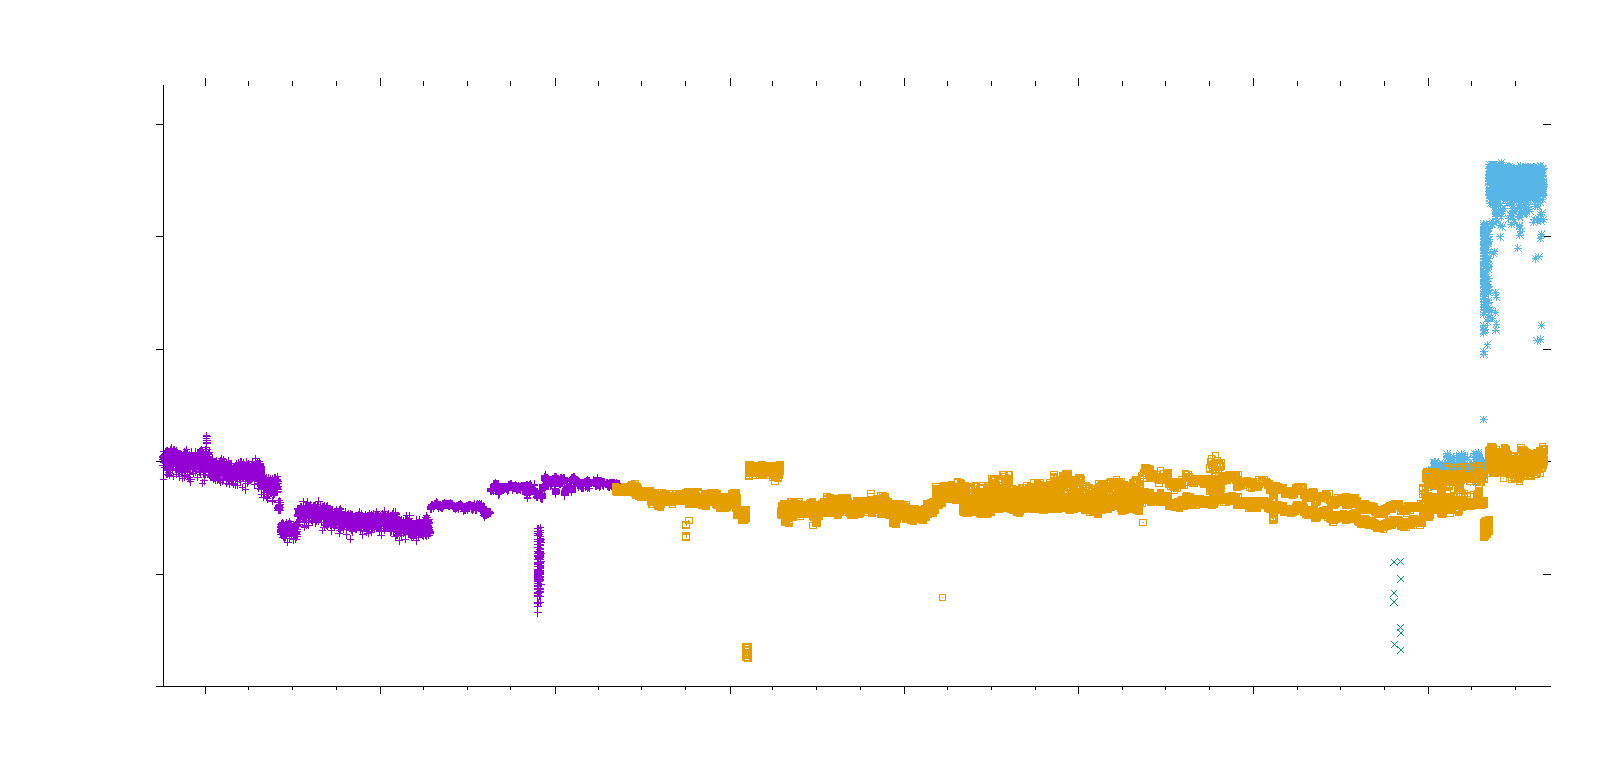
\includegraphics[width={756.00bp},height={360.00bp}]{gnuplot/tcp-0,1,2,3}}%
    \gplfronttext
  \end{picture}%
\endgroup

    \end{adjustbox}
  };
  \path[red,font=\small]
    (2.3,1.5) node [anchor=south] {meltdown} node [anchor=center] {spectre}
    (4.8,1.1) node [anchor=south] {buggy} node [anchor=center] {timer}
    (6.8,3.5) node [anchor=south] {delay} node [anchor=center] {second}
	node [anchor=north] {ACK}
    (9,3) node [anchor=south] {parallel} node [anchor=center] {IP input}
    (10.5,3) node [anchor=south] {TSO}
    (11.5,1.8) node [anchor=south] {fine} node [anchor=center] {grained}
	node [anchor=north] {locking}
    (12.8,3.3) node [anchor=south] {parallel} node [anchor=center] {TCP output}
    (13.2,1.6) node [anchor=south] {per} node [anchor=center] {packet}
	node [anchor=north] {lock}
    (13.5,5.8) node [anchor=south] {parallel} node [anchor=center] {TCP input}
  ;
\end{tikzpicture}
\end{frame}

\section{Packet Processing}

\subsection{Network Protocol Stack}
\subsection{Network Protocol Stack}
\begin{frame}{Network Protocol Stack}
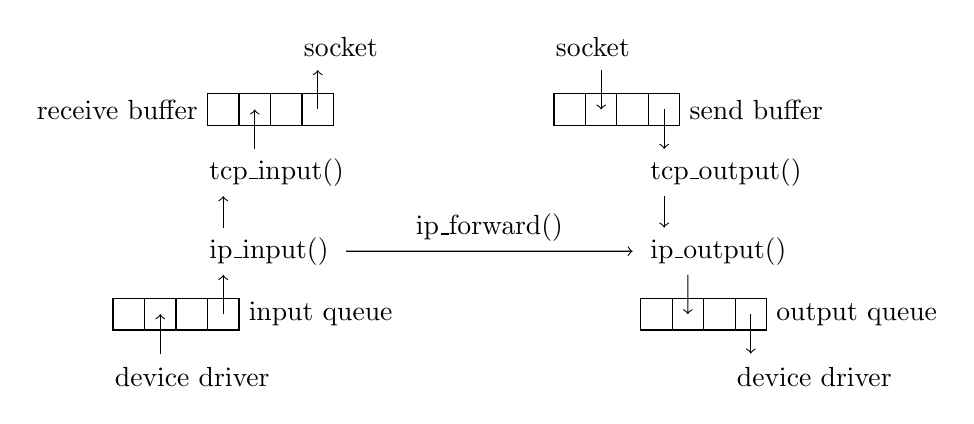
\begin{tikzpicture}
  \draw (0,0)
    node (idd) [right] {device driver} ++(.1,.6)
    rectangle ++(.4,.4) rectangle ++(.4,-.4)
    rectangle ++(.4,.4) rectangle ++(.4,-.4) ++(0,.2)
    node (iq) [right] {input queue} ++(-.5,.8)
    node (ii) [right] {ip\_input()} ++(0,1.0)
    node (ti) [right] {tcp\_input()} ++(.1,.8)
    node (rb) [left] {receive buffer} ++(0,-.2)
    rectangle ++(.4,.4) rectangle ++(.4,-.4)
    rectangle ++(.4,.4) rectangle ++(.4,-.4) ++(-.5,1.0)
    node (iso) [right] {socket} ++(3.2,0)

    node (oso) [right] {socket} ++(.1,-.6)
    rectangle ++(.4,-.4) rectangle ++(.4,.4)
    rectangle ++(.4,-.4) rectangle ++(.4,.4) ++(0,-.2)
    node (sb) [right] {send buffer} ++(-.5,-.8)
    node (to) [right] {tcp\_output()} ++(0,-1.0)
    node (io) [right] {ip\_output()} ++(0,-.6)
    rectangle ++(.4,-.4) rectangle ++(.4,.4)
    rectangle ++(.4,-.4) rectangle ++(.4,.4) ++(0,-.2)
    node (oq) [right] {output queue} ++(-.5,-.8)
    node (odd) [right] {device driver}
    ;
  \path (node cs:name=idd,anchor=west) +(.3+1*.4,.3) coordinate (iddo) {};
  \path (node cs:name=iq,anchor=west) +(-.2-2*.4,0) coordinate (iqi) {};
  \draw[->] (iddo) -- (iqi);
  \path (node cs:name=iq,anchor=west) +(-.2,0) coordinate (iqo) {};
  \path (node cs:name=ii,anchor=west) +(.3,-.3) coordinate (iii) {};
  \draw[->] (iqo) -- (iii);
  \path (node cs:name=ii,anchor=west) +(.3,.3) coordinate (iio) {};
  \path (node cs:name=ti,anchor=west) +(.3,-.3) coordinate (tii) {};
  \draw[->] (iio) -- (tii);
  \path (node cs:name=ti,anchor=west) +(.3+1*.4,.3) coordinate (iti) {};
  \path (node cs:name=rb,anchor=east) +(.2+1*.4,0) coordinate (rbi) {};
  \draw[->] (iti) -- (rbi);
  \path (node cs:name=rb,anchor=east) +(.2+3*.4,0) coordinate (rbo) {};
  \path (node cs:name=iso,anchor=west) +(.3,-.3) coordinate (isoi) {};
  \draw[->] (rbo) -- (isoi);

  \path (node cs:name=oso,anchor=west) +(.3+1*.4,-.3) coordinate (osoo) {};
  \path (node cs:name=sb,anchor=west) +(-.2-2*.4,0) coordinate (sbi) {};
  \draw[->] (osoo) -- (sbi);
  \path (node cs:name=sb,anchor=west) +(-.2,0) coordinate (sbo) {};
  \path (node cs:name=to,anchor=west) +(.3,.3) coordinate (toi) {};
  \draw[->] (sbo) -- (toi);
  \path (node cs:name=to,anchor=west) +(.3,-.3) coordinate (too) {};
  \path (node cs:name=io,anchor=west) +(.3,.3) coordinate (ioi) {};
  \draw[->] (too) -- (ioi);
  \path (node cs:name=io,anchor=west) +(.6,-.3) coordinate (ioo) {};
  \path (node cs:name=oq,anchor=west) +(-.2-2*.4,0) coordinate (oqi) {};
  \draw[->] (ioo) -- (oqi);
  \path (node cs:name=oq,anchor=west) +(-.2,0) coordinate (oqo) {};
  \path (node cs:name=odd,anchor=west) +(.3,.3) coordinate (oddi) {};
  \draw[->] (oqo) -- (oddi);

  \path (node cs:name=ii,anchor=east) +(.1,0) coordinate (ifo) {};
  \path (node cs:name=io,anchor=west) +(-.1,0) coordinate (ifi) {};
  \draw[->] (ifo) -- (ifi) node [midway,above] {ip\_forward()};
\end{tikzpicture}
\end{frame}

\subsection{Towards Parallel Processing}
\begin{frame}{Towards Parallel Processing, 2024}
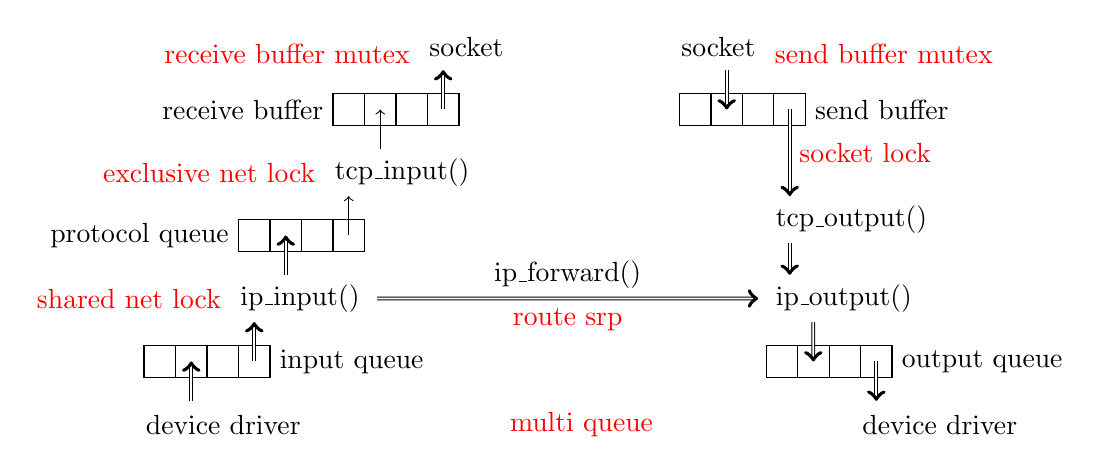
\begin{tikzpicture}
  \draw (0,0)
    node (idd) [right] {device driver} ++(.1,.6)
    rectangle ++(.4,.4) rectangle ++(.4,-.4)
    rectangle ++(.4,.4) rectangle ++(.4,-.4) ++(0,.2)
    node (iq) [right] {input queue} ++(-.5,.8)
    node (ii) [right] {ip\_input()} ++(.1,.8)
    node (pq) [left] {protocol queue} ++(0,-.2)
    rectangle ++(.4,.4) rectangle ++(.4,-.4)
    rectangle ++(.4,.4) rectangle ++(.4,-.4) ++(-.5,1.0)
    node (ti) [right] {tcp\_input()} ++(.1,.8)
    node (rb) [left] {receive buffer} ++(0,-.2)
    rectangle ++(.4,.4) rectangle ++(.4,-.4)
    rectangle ++(.4,.4) rectangle ++(.4,-.4) ++(-.5,1.0)
    node (iso) [right] {socket} ++(3.2,0)

    node (oso) [right] {socket} ++(.1,-.6)
    rectangle ++(.4,-.4) rectangle ++(.4,.4)
    rectangle ++(.4,-.4) rectangle ++(.4,.4) ++(0,-.2)
    node (sb) [right] {send buffer} ++(-.5,-1.4)
    node (to) [right] {tcp\_output()} ++(0,-1.0)
    node (io) [right] {ip\_output()} ++(0,-.6)
    rectangle ++(.4,-.4) rectangle ++(.4,.4)
    rectangle ++(.4,-.4) rectangle ++(.4,.4) ++(0,-.2)
    node (oq) [right] {output queue} ++(-.5,-.8)
    node (odd) [right] {device driver}
    ;
  \path (node cs:name=idd,anchor=west) +(.3+1*.4,.3) coordinate (iddo) {};
  \path (node cs:name=iq,anchor=west) +(-.2-2*.4,0) coordinate (iqi) {};
  \draw[->,double] (iddo) -- (iqi);
  \path (node cs:name=iq,anchor=west) +(-.2,0) coordinate (iqo) {};
  \path (node cs:name=ii,anchor=west) +(.3,-.3) coordinate (iii) {};
  \draw[->,double] (iqo) -- (iii);
  \path (node cs:name=ii,anchor=west) +(.3+1*.4,.3) coordinate (iio) {};
  \path (node cs:name=pq,anchor=east) +(.2+1*.4,0) coordinate (pqi) {};
  \draw[->,double] (iio) -- (pqi);
  \path (node cs:name=pq,anchor=east) +(.2+3*.4,0) coordinate (pqo) {};
  \path (node cs:name=ti,anchor=west) +(.3,-.3) coordinate (tii) {};
  \draw[->] (pqo) -- (tii);
  \path (node cs:name=ti,anchor=west) +(.3+1*.4,.3) coordinate (iti) {};
  \path (node cs:name=rb,anchor=east) +(.2+1*.4,0) coordinate (rbi) {};
  \draw[->] (iti) -- (rbi);
  \path (node cs:name=rb,anchor=east) +(.2+3*.4,0) coordinate (rbo) {};
  \path (node cs:name=iso,anchor=west) +(.3,-.3) coordinate (isoi) {};
  \draw[->,double] (rbo) -- (isoi);

  \path (node cs:name=oso,anchor=west) +(.3+1*.4,-.3) coordinate (osoo) {};
  \path (node cs:name=sb,anchor=west) +(-.2-2*.4,0) coordinate (sbi) {};
  \draw[->,double] (osoo) -- (sbi);
  \path (node cs:name=sb,anchor=west) +(-.2,0) coordinate (sbo) {};
  \path (node cs:name=to,anchor=west) +(.3,.3) coordinate (toi) {};
  \draw[->,double] (sbo) -- (toi);
  \path (node cs:name=to,anchor=west) +(.3,-.3) coordinate (too) {};
  \path (node cs:name=io,anchor=west) +(.3,.3) coordinate (ioi) {};
  \draw[->,double] (too) -- (ioi);
  \path (node cs:name=io,anchor=west) +(.6,-.3) coordinate (ioo) {};
  \path (node cs:name=oq,anchor=west) +(-.2-2*.4,0) coordinate (oqi) {};
  \draw[->,double] (ioo) -- (oqi);
  \path (node cs:name=oq,anchor=west) +(-.2,0) coordinate (oqo) {};
  \path (node cs:name=odd,anchor=west) +(.3,.3) coordinate (oddi) {};
  \draw[->,double] (oqo) -- (oddi);

  \path (node cs:name=ii,anchor=east) +(.1,0) coordinate (ifo) {};
  \path (node cs:name=io,anchor=west) +(-.1,0) coordinate (ifi) {};
  \draw[->,double] (ifo) -- (ifi) node [midway,above] {ip\_forward()};

  \draw[red] (node cs:name=iso,anchor=west) +(0,-.1)
    node [left] {receive buffer mutex};
  \draw[red] (node cs:name=oso,anchor=east) +(0,-.1)
    node [right] {send buffer mutex};
  \draw[red] (node cs:name=ti,anchor=west) node [left] {exclusive net lock};
  \path (sbo) -- (toi) node [red,midway,right] {socket lock};
  \draw[red] (node cs:name=ii,anchor=west) node [left] {shared net lock};
  \path (ifo) -- (ifi) node [red,midway,below] {route srp};
  \path (idd) -- (odd) node [red,midway] {multi queue};
\end{tikzpicture}
\end{frame}

\subsection{Parallel UDP Input}
\begin{frame}{Parallel UDP Input, 2024}
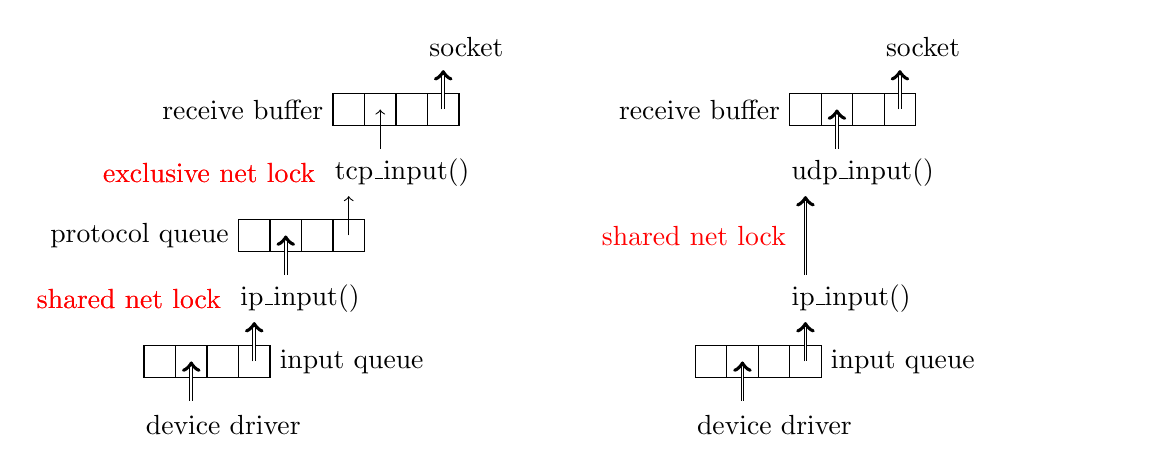
\begin{tikzpicture}
  \draw (0,0)
    node (idd) [right] {device driver} ++(.1,.6)
    rectangle ++(.4,.4) rectangle ++(.4,-.4)
    rectangle ++(.4,.4) rectangle ++(.4,-.4) ++(0,.2)
    node (iq) [right] {input queue} ++(-.5,.8)
    node (ii) [right] {ip\_input()} ++(.1,.8)
    node (pq) [left] {protocol queue} ++(0,-.2)
    rectangle ++(.4,.4) rectangle ++(.4,-.4)
    rectangle ++(.4,.4) rectangle ++(.4,-.4) ++(-.5,1.0)
    node (ti) [right] {tcp\_input()} ++(.1,.8)
    node (rb) [left] {receive buffer} ++(0,-.2)
    rectangle ++(.4,.4) rectangle ++(.4,-.4)
    rectangle ++(.4,.4) rectangle ++(.4,-.4) ++(-.5,1.0)
    node (iso) [right] {socket} ++(3.2,0)
    ;
  \path (node cs:name=idd,anchor=west) +(.3+1*.4,.3) coordinate (iddo) {};
  \path (node cs:name=iq,anchor=west) +(-.2-2*.4,0) coordinate (iqi) {};
  \draw[->,double] (iddo) -- (iqi);
  \path (node cs:name=iq,anchor=west) +(-.2,0) coordinate (iqo) {};
  \path (node cs:name=ii,anchor=west) +(.3,-.3) coordinate (iii) {};
  \draw[->,double] (iqo) -- (iii);
  \path (node cs:name=ii,anchor=west) +(.3+1*.4,.3) coordinate (iio) {};
  \path (node cs:name=pq,anchor=east) +(.2+1*.4,0) coordinate (pqi) {};
  \draw[->,double] (iio) -- (pqi);
  \path (node cs:name=pq,anchor=east) +(.2+3*.4,0) coordinate (pqo) {};
  \path (node cs:name=ti,anchor=west) +(.3,-.3) coordinate (tii) {};
  \draw[->] (pqo) -- (tii);
  \path (node cs:name=ti,anchor=west) +(.3+1*.4,.3) coordinate (iti) {};
  \path (node cs:name=rb,anchor=east) +(.2+1*.4,0) coordinate (rbi) {};
  \draw[->] (iti) -- (rbi);
  \path (node cs:name=rb,anchor=east) +(.2+3*.4,0) coordinate (rbo) {};
  \path (node cs:name=iso,anchor=west) +(.3,-.3) coordinate (isoi) {};
  \draw[->,double] (rbo) -- (isoi);

  \draw[red] (node cs:name=ti,anchor=west) node [left] {exclusive net lock};
  \draw[red] (node cs:name=ii,anchor=west) node [left] {shared net lock};

  \draw (7,0)
    node (udd) [right] {device driver} ++(.1,.6)
    rectangle ++(.4,.4) rectangle ++(.4,-.4)
    rectangle ++(.4,.4) rectangle ++(.4,-.4) ++(0,.2)
    node (uiq) [right] {input queue} ++(-.5,.8)
    node (uii) [right] {ip\_input()} ++(0,1.6)
    node (ui) [right] {udp\_input()} ++(.1,.8)
    node (urb) [left] {receive buffer} ++(0,-.2)
    rectangle ++(.4,.4) rectangle ++(.4,-.4)
    rectangle ++(.4,.4) rectangle ++(.4,-.4) ++(-.5,1.0)
    node (uso) [right] {socket} ++(3.2,0)
    ;
  \path (node cs:name=udd,anchor=west) +(.3+1*.4,.3) coordinate (uddo) {};
  \path (node cs:name=uiq,anchor=west) +(-.2-2*.4,0) coordinate (uiqi) {};
  \draw[->,double] (uddo) -- (uiqi);
  \path (node cs:name=uiq,anchor=west) +(-.2,0) coordinate (uiqo) {};
  \path (node cs:name=uii,anchor=west) +(.3,-.3) coordinate (uiii) {};
  \draw[->,double] (uiqo) -- (uiii);
  \path (node cs:name=uii,anchor=west) +(.3,.3) coordinate (uiio) {};
  \path (node cs:name=ui,anchor=west) +(.3,-.3) coordinate (uii) {};
  \draw[->,double] (uiio) -- (uii) node [midway] (upi) {};
  \path (node cs:name=ui,anchor=west) +(.3+1*.4,.3) coordinate (iui) {};
  \path (node cs:name=urb,anchor=east) +(.2+1*.4,0) coordinate (urbi) {};
  \draw[->,double] (iui) -- (urbi);
  \path (node cs:name=urb,anchor=east) +(.2+3*.4,0) coordinate (urbo) {};
  \path (node cs:name=uso,anchor=west) +(.3,-.3) coordinate (usoi) {};
  \draw[->,double] (urbo) -- (usoi);

  \draw[red] (node cs:name=ti,anchor=west) node [left] {exclusive net lock};
  \draw[red] (node cs:name=ii,anchor=west) node [left] {shared net lock};
  \draw[red] (node cs:name=upi,anchor=west) node [left] {shared net lock};
\end{tikzpicture}
\end{frame}

\subsection{Parallel TCP Input}
\begin{frame}{Parallel TCP Input, 2025}
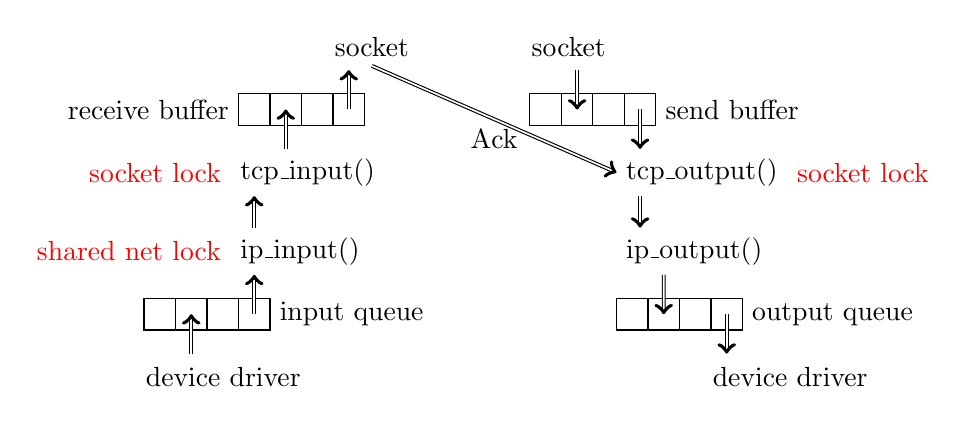
\begin{tikzpicture}
  \draw (0,0)
    node (idd) [right] {device driver} ++(.1,.6)
    rectangle ++(.4,.4) rectangle ++(.4,-.4)
    rectangle ++(.4,.4) rectangle ++(.4,-.4) ++(0,.2)
    node (iq) [right] {input queue} ++(-.5,.8)
    node (ii) [right] {ip\_input()} ++(0,1.0)
    node (ti) [right] {tcp\_input()} ++(.1,.8)
    node (rb) [left] {receive buffer} ++(0,-.2)
    rectangle ++(.4,.4) rectangle ++(.4,-.4)
    rectangle ++(.4,.4) rectangle ++(.4,-.4) ++(-.5,1.0)
    node (iso) [right] {socket} ++(2.5,0)

    node (oso) [right] {socket} ++(.1,-.6)
    rectangle ++(.4,-.4) rectangle ++(.4,.4)
    rectangle ++(.4,-.4) rectangle ++(.4,.4) ++(0,-.2)
    node (sb) [right] {send buffer} ++(-.5,-.8)
    node (to) [right] {tcp\_output()} ++(0,-1.0)
    node (io) [right] {ip\_output()} ++(0,-.6)
    rectangle ++(.4,-.4) rectangle ++(.4,.4)
    rectangle ++(.4,-.4) rectangle ++(.4,.4) ++(0,-.2)
    node (oq) [right] {output queue} ++(-.5,-.8)
    node (odd) [right] {device driver}
    ;
  \path (node cs:name=idd,anchor=west) +(.3+1*.4,.3) coordinate (iddo) {};
  \path (node cs:name=iq,anchor=west) +(-.2-2*.4,0) coordinate (iqi) {};
  \draw[->,double] (iddo) -- (iqi);
  \path (node cs:name=iq,anchor=west) +(-.2,0) coordinate (iqo) {};
  \path (node cs:name=ii,anchor=west) +(.3,-.3) coordinate (iii) {};
  \draw[->,double] (iqo) -- (iii);
  \path (node cs:name=ii,anchor=west) +(.3,.3) coordinate (iio) {};
  \path (node cs:name=ti,anchor=west) +(.3,-.3) coordinate (tii) {};
  \draw[->,double] (iio) -- (tii);
  \path (node cs:name=ti,anchor=west) +(.3+1*.4,.3) coordinate (iti) {};
  \path (node cs:name=rb,anchor=east) +(.2+1*.4,0) coordinate (rbi) {};
  \draw[->,double] (iti) -- (rbi);
  \path (node cs:name=rb,anchor=east) +(.2+3*.4,0) coordinate (rbo) {};
  \path (node cs:name=iso,anchor=west) +(.3,-.3) coordinate (isoi) {};
  \draw[->,double] (rbo) -- (isoi);

  \path (node cs:name=oso,anchor=west) +(.3+1*.4,-.3) coordinate (osoo) {};
  \path (node cs:name=sb,anchor=west) +(-.2-2*.4,0) coordinate (sbi) {};
  \draw[->,double] (osoo) -- (sbi);
  \path (node cs:name=sb,anchor=west) +(-.2,0) coordinate (sbo) {};
  \path (node cs:name=to,anchor=west) +(.3,.3) coordinate (toi) {};
  \draw[->,double] (sbo) -- (toi);
  \path (node cs:name=to,anchor=west) +(.3,-.3) coordinate (too) {};
  \path (node cs:name=io,anchor=west) +(.3,.3) coordinate (ioi) {};
  \draw[->,double] (too) -- (ioi);
  \path (node cs:name=io,anchor=west) +(.6,-.3) coordinate (ioo) {};
  \path (node cs:name=oq,anchor=west) +(-.2-2*.4,0) coordinate (oqi) {};
  \draw[->,double] (ioo) -- (oqi);
  \path (node cs:name=oq,anchor=west) +(-.2,0) coordinate (oqo) {};
  \path (node cs:name=odd,anchor=west) +(.3,.3) coordinate (oddi) {};
  \draw[->,double] (oqo) -- (oddi);

  \path (node cs:name=iso,anchor=south) coordinate (tro) {};
  \path (node cs:name=to,anchor=west) coordinate (tri) {};
  \draw[->,double] (tro) -- (tri) node [midway,below] {Ack};

  \draw[red] (node cs:name=ti,anchor=west) node [left] {socket lock};
  \draw[red] (node cs:name=to,anchor=east) node [right] {socket lock};
  \draw[red] (node cs:name=ii,anchor=west) node [left] {shared net lock};
\end{tikzpicture}
\end{frame}

\section{Performance}

\subsection{Exclusive TCP Receive Single Stream}
\begin{frame}{Exclusive TCP Receive Single Stream}
    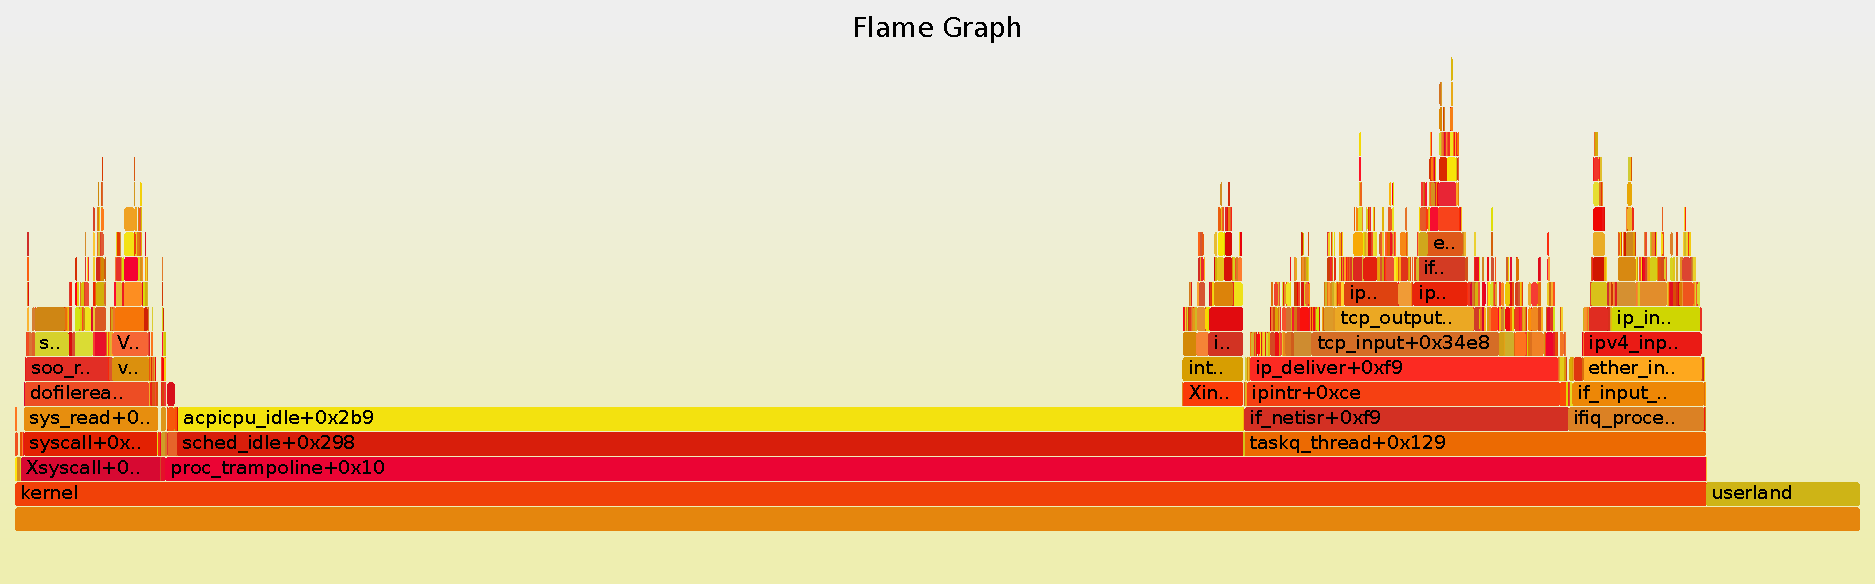
\includegraphics[width=\textwidth]{kstack/sys-tcp-input-solock-rev-single.pdf}
\end{frame}

\subsection{Parallel TCP Receive Single Stream}
\begin{frame}{Parallel TCP Receive Single Stream}
\begin{tikzpicture}
  \path (0,0) node [anchor=south west] {
    \begin{adjustbox}{width=\textwidth-0\baselineskip}
      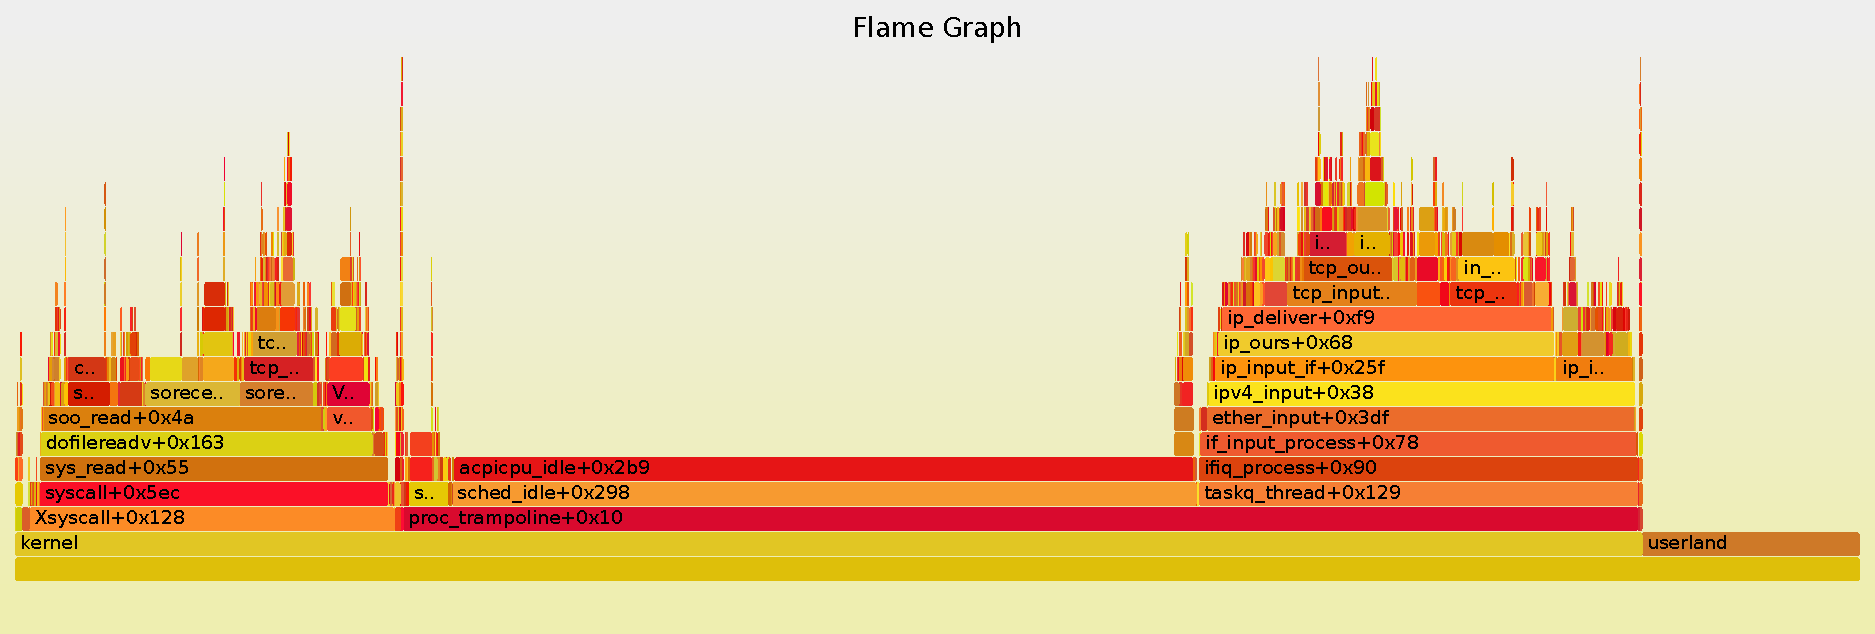
\includegraphics[width=\textwidth]{kstack/sys-tcp-mpinput-rev-single.pdf}
    \end{adjustbox}
  };
  \path[ellipse,black,thick]
    (1.6,2.15) node [draw,minimum width=.8cm,minimum height=.2cm] {}
    (11.25,3.05) node [draw,minimum width=.5cm,minimum height=.2cm] {}
  ;
\end{tikzpicture}
\end{frame}

\subsection{Parallel TCP Input, Socket Lock per Thread}
\begin{frame}{Parallel TCP Input, Socket Lock per Thread}
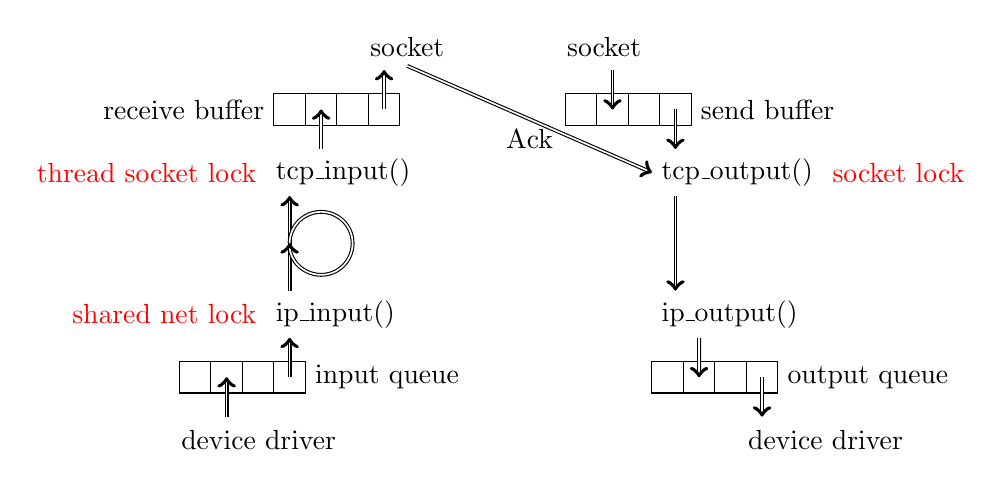
\begin{tikzpicture}
  \draw (0,0)
    node (idd) [right] {device driver} ++(.1,.6)
    rectangle ++(.4,.4) rectangle ++(.4,-.4)
    rectangle ++(.4,.4) rectangle ++(.4,-.4) ++(0,.2)
    node (iq) [right] {input queue} ++(-.5,.8)
    node (ii) [right] {ip\_input()} ++(0,1.8)
    node (ti) [right] {tcp\_input()} ++(.1,.8)
    node (rb) [left] {receive buffer} ++(0,-.2)
    rectangle ++(.4,.4) rectangle ++(.4,-.4)
    rectangle ++(.4,.4) rectangle ++(.4,-.4) ++(-.5,1.0)
    node (iso) [right] {socket} ++(2.5,0)

    node (oso) [right] {socket} ++(.1,-.6)
    rectangle ++(.4,-.4) rectangle ++(.4,.4)
    rectangle ++(.4,-.4) rectangle ++(.4,.4) ++(0,-.2)
    node (sb) [right] {send buffer} ++(-.5,-0.8)
    node (to) [right] {tcp\_output()} ++(0,-1.8)
    node (io) [right] {ip\_output()} ++(0,-.6)
    rectangle ++(.4,-.4) rectangle ++(.4,.4)
    rectangle ++(.4,-.4) rectangle ++(.4,.4) ++(0,-.2)
    node (oq) [right] {output queue} ++(-.5,-.8)
    node (odd) [right] {device driver}
    ;
  \path (node cs:name=idd,anchor=west) +(.3+1*.4,.3) coordinate (iddo) {};
  \path (node cs:name=iq,anchor=west) +(-.2-2*.4,0) coordinate (iqi) {};
  \draw[->,double] (iddo) -- (iqi);
  \path (node cs:name=iq,anchor=west) +(-.2,0) coordinate (iqo) {};
  \path (node cs:name=ii,anchor=west) +(.3,-.3) coordinate (iii) {};
  \draw[->,double] (iqo) -- (iii);
  \path (node cs:name=ii,anchor=west) +(.3,.3) coordinate (iio) {};
  \path (node cs:name=ti,anchor=west) +(.3,-.3) coordinate (tii) {};
  \draw[->,double] (iio) -- (tii) node (tt) [midway] {};
  \draw[->,double] (node cs:name=tt) arc [start angle=360,end angle=0,radius=-.4cm];
  \path (node cs:name=ti,anchor=west) +(.3+1*.4,.3) coordinate (iti) {};
  \path (node cs:name=rb,anchor=east) +(.2+1*.4,0) coordinate (rbi) {};
  \draw[->,double] (iti) -- (rbi);
  \path (node cs:name=rb,anchor=east) +(.2+3*.4,0) coordinate (rbo) {};
  \path (node cs:name=iso,anchor=west) +(.3,-.3) coordinate (isoi) {};
  \draw[->,double] (rbo) -- (isoi);

  \path (node cs:name=oso,anchor=west) +(.3+1*.4,-.3) coordinate (osoo) {};
  \path (node cs:name=sb,anchor=west) +(-.2-2*.4,0) coordinate (sbi) {};
  \draw[->,double] (osoo) -- (sbi);
  \path (node cs:name=sb,anchor=west) +(-.2,0) coordinate (sbo) {};
  \path (node cs:name=to,anchor=west) +(.3,.3) coordinate (toi) {};
  \draw[->,double] (sbo) -- (toi);
  \path (node cs:name=to,anchor=west) +(.3,-.3) coordinate (too) {};
  \path (node cs:name=io,anchor=west) +(.3,.3) coordinate (ioi) {};
  \draw[->,double] (too) -- (ioi);
  \path (node cs:name=io,anchor=west) +(.6,-.3) coordinate (ioo) {};
  \path (node cs:name=oq,anchor=west) +(-.2-2*.4,0) coordinate (oqi) {};
  \draw[->,double] (ioo) -- (oqi);
  \path (node cs:name=oq,anchor=west) +(-.2,0) coordinate (oqo) {};
  \path (node cs:name=odd,anchor=west) +(.3,.3) coordinate (oddi) {};
  \draw[->,double] (oqo) -- (oddi);

  \path (node cs:name=iso,anchor=south) coordinate (tro) {};
  \path (node cs:name=to,anchor=west) coordinate (tri) {};
  \draw[->,double] (tro) -- (tri) node [midway,below] {Ack};


  \draw[red] (node cs:name=ti,anchor=west) node [left] {thread socket lock};
  \draw[red] (node cs:name=to,anchor=east) node [right] {socket lock};
  \draw[red] (node cs:name=ii,anchor=west) node [left] {shared net lock};
\end{tikzpicture}
\end{frame}

\subsection{Variants for TCP Input}
\begin{frame}{Variants for TCP Input}
\begin{tikzpicture}
  \path (0,0) node [anchor=south west] {
    \begin{adjustbox}{width=\textwidth-0\baselineskip}
      % GNUPLOT: LaTeX picture with Postscript
\begingroup
  \makeatletter
  \providecommand\color[2][]{%
    \GenericError{(gnuplot) \space\space\space\@spaces}{%
      Package color not loaded in conjunction with
      terminal option `colourtext'%
    }{See the gnuplot documentation for explanation.%
    }{Either use 'blacktext' in gnuplot or load the package
      color.sty in LaTeX.}%
    \renewcommand\color[2][]{}%
  }%
  \providecommand\includegraphics[2][]{%
    \GenericError{(gnuplot) \space\space\space\@spaces}{%
      Package graphicx or graphics not loaded%
    }{See the gnuplot documentation for explanation.%
    }{The gnuplot epslatex terminal needs graphicx.sty or graphics.sty.}%
    \renewcommand\includegraphics[2][]{}%
  }%
  \providecommand\rotatebox[2]{#2}%
  \@ifundefined{ifGPcolor}{%
    \newif\ifGPcolor
    \GPcolortrue
  }{}%
  \@ifundefined{ifGPblacktext}{%
    \newif\ifGPblacktext
    \GPblacktexttrue
  }{}%
  % define a \g@addto@macro without @ in the name:
  \let\gplgaddtomacro\g@addto@macro
  % define empty templates for all commands taking text:
  \gdef\gplbacktext{}%
  \gdef\gplfronttext{}%
  \makeatother
  \ifGPblacktext
    % no textcolor at all
    \def\colorrgb#1{}%
    \def\colorgray#1{}%
  \else
    % gray or color?
    \ifGPcolor
      \def\colorrgb#1{\color[rgb]{#1}}%
      \def\colorgray#1{\color[gray]{#1}}%
      \expandafter\def\csname LTw\endcsname{\color{white}}%
      \expandafter\def\csname LTb\endcsname{\color{black}}%
      \expandafter\def\csname LTa\endcsname{\color{black}}%
      \expandafter\def\csname LT0\endcsname{\color[rgb]{1,0,0}}%
      \expandafter\def\csname LT1\endcsname{\color[rgb]{0,1,0}}%
      \expandafter\def\csname LT2\endcsname{\color[rgb]{0,0,1}}%
      \expandafter\def\csname LT3\endcsname{\color[rgb]{1,0,1}}%
      \expandafter\def\csname LT4\endcsname{\color[rgb]{0,1,1}}%
      \expandafter\def\csname LT5\endcsname{\color[rgb]{1,1,0}}%
      \expandafter\def\csname LT6\endcsname{\color[rgb]{0,0,0}}%
      \expandafter\def\csname LT7\endcsname{\color[rgb]{1,0.3,0}}%
      \expandafter\def\csname LT8\endcsname{\color[rgb]{0.5,0.5,0.5}}%
    \else
      % gray
      \def\colorrgb#1{\color{black}}%
      \def\colorgray#1{\color[gray]{#1}}%
      \expandafter\def\csname LTw\endcsname{\color{white}}%
      \expandafter\def\csname LTb\endcsname{\color{black}}%
      \expandafter\def\csname LTa\endcsname{\color{black}}%
      \expandafter\def\csname LT0\endcsname{\color{black}}%
      \expandafter\def\csname LT1\endcsname{\color{black}}%
      \expandafter\def\csname LT2\endcsname{\color{black}}%
      \expandafter\def\csname LT3\endcsname{\color{black}}%
      \expandafter\def\csname LT4\endcsname{\color{black}}%
      \expandafter\def\csname LT5\endcsname{\color{black}}%
      \expandafter\def\csname LT6\endcsname{\color{black}}%
      \expandafter\def\csname LT7\endcsname{\color{black}}%
      \expandafter\def\csname LT8\endcsname{\color{black}}%
    \fi
  \fi
    \setlength{\unitlength}{0.0500bp}%
    \ifx\gptboxheight\undefined%
      \newlength{\gptboxheight}%
      \newlength{\gptboxwidth}%
      \newsavebox{\gptboxtext}%
    \fi%
    \setlength{\fboxrule}{0.5pt}%
    \setlength{\fboxsep}{1pt}%
    \definecolor{tbcol}{rgb}{1,1,1}%
\begin{picture}(15120.00,7200.00)%
    \gplgaddtomacro\gplbacktext{%
      \csname LTb\endcsname%%
      \put(1078,767){\makebox(0,0)[r]{\strut{}$0$}}%
      \put(1078,1357){\makebox(0,0)[r]{\strut{}$1\times10^{9}$}}%
      \put(1078,1946){\makebox(0,0)[r]{\strut{}$2\times10^{9}$}}%
      \put(1078,2536){\makebox(0,0)[r]{\strut{}$3\times10^{9}$}}%
      \put(1078,3126){\makebox(0,0)[r]{\strut{}$4\times10^{9}$}}%
      \put(1078,3716){\makebox(0,0)[r]{\strut{}$5\times10^{9}$}}%
      \put(1078,4305){\makebox(0,0)[r]{\strut{}$6\times10^{9}$}}%
      \put(1078,4895){\makebox(0,0)[r]{\strut{}$7\times10^{9}$}}%
      \put(1078,5485){\makebox(0,0)[r]{\strut{}$8\times10^{9}$}}%
      \put(1078,6074){\makebox(0,0)[r]{\strut{}$9\times10^{9}$}}%
      \put(1273,484){\makebox(0,0){\strut{}2025-01-25}}%
      \put(3950,484){\makebox(0,0){\strut{}2025-01-26}}%
      \put(6628,484){\makebox(0,0){\strut{}2025-01-26}}%
      \put(9305,484){\makebox(0,0){\strut{}2025-01-26}}%
      \put(11983,484){\makebox(0,0){\strut{}2025-01-26}}%
      \put(14660,484){\makebox(0,0){\strut{}2025-01-26}}%
    }%
    \gplgaddtomacro\gplfronttext{%
      \csname LTb\endcsname%%
      \put(209,3653){\rotatebox{-270}{\makebox(0,0){\strut{}bits/sec}}}%
      \put(7966,154){\makebox(0,0){\strut{}Checkout (date)}}%
      \csname LTb\endcsname%%
      \put(7966,6869){\makebox(0,0){\strut{}TCP Performance}}%
    }%
    \gplbacktext
    \put(0,0){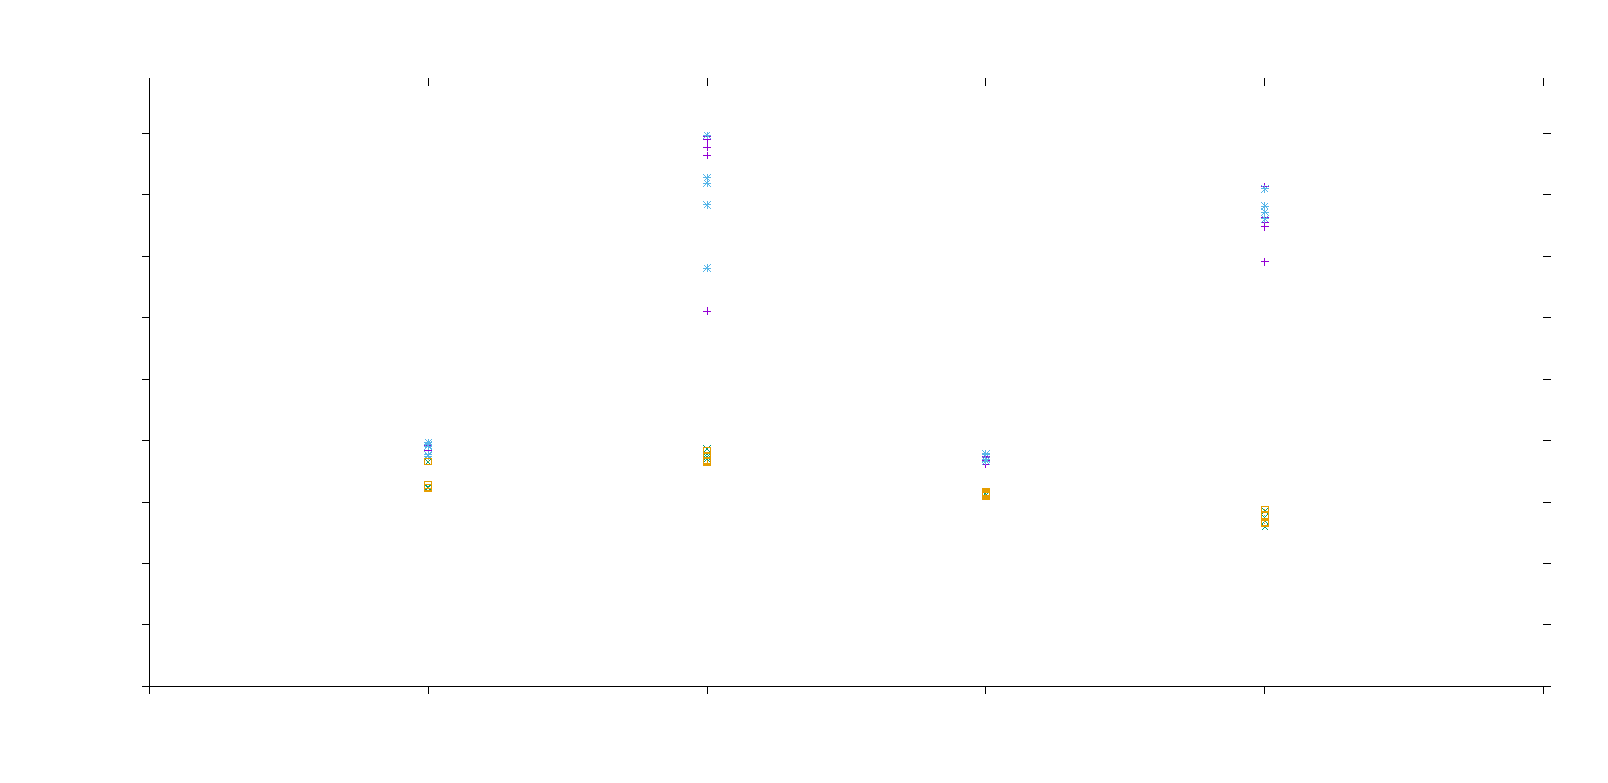
\includegraphics[width={756.00bp},height={360.00bp}]{gnuplot/2025-01-26T17:08:00Z-tcp-0,1,2,3}}%
    \gplfronttext
  \end{picture}%
\endgroup

    \end{adjustbox}
  };
  \path[red,font=\small]
    (3.8,1.5) node [anchor=south] {exclusive} node [anchor=center] {net lock}
    ++(2.4,0) node [anchor=south] {parallel} node [anchor=center] {TCP input}
	node [anchor=north] {per thread lock}
    ++(2.4,0) node [anchor=south] {cost of} node [anchor=center] {socket lock}
    ++(2.4,0) node [anchor=south] {parallel} node [anchor=center] {TCP input}
  ;
\end{tikzpicture}
\end{frame}

\subsection{TCP Receive Parallel Stream, Socket Lock per Thread}
\begin{frame}{TCP Receive Parallel Stream, Socket Lock per Thread}
    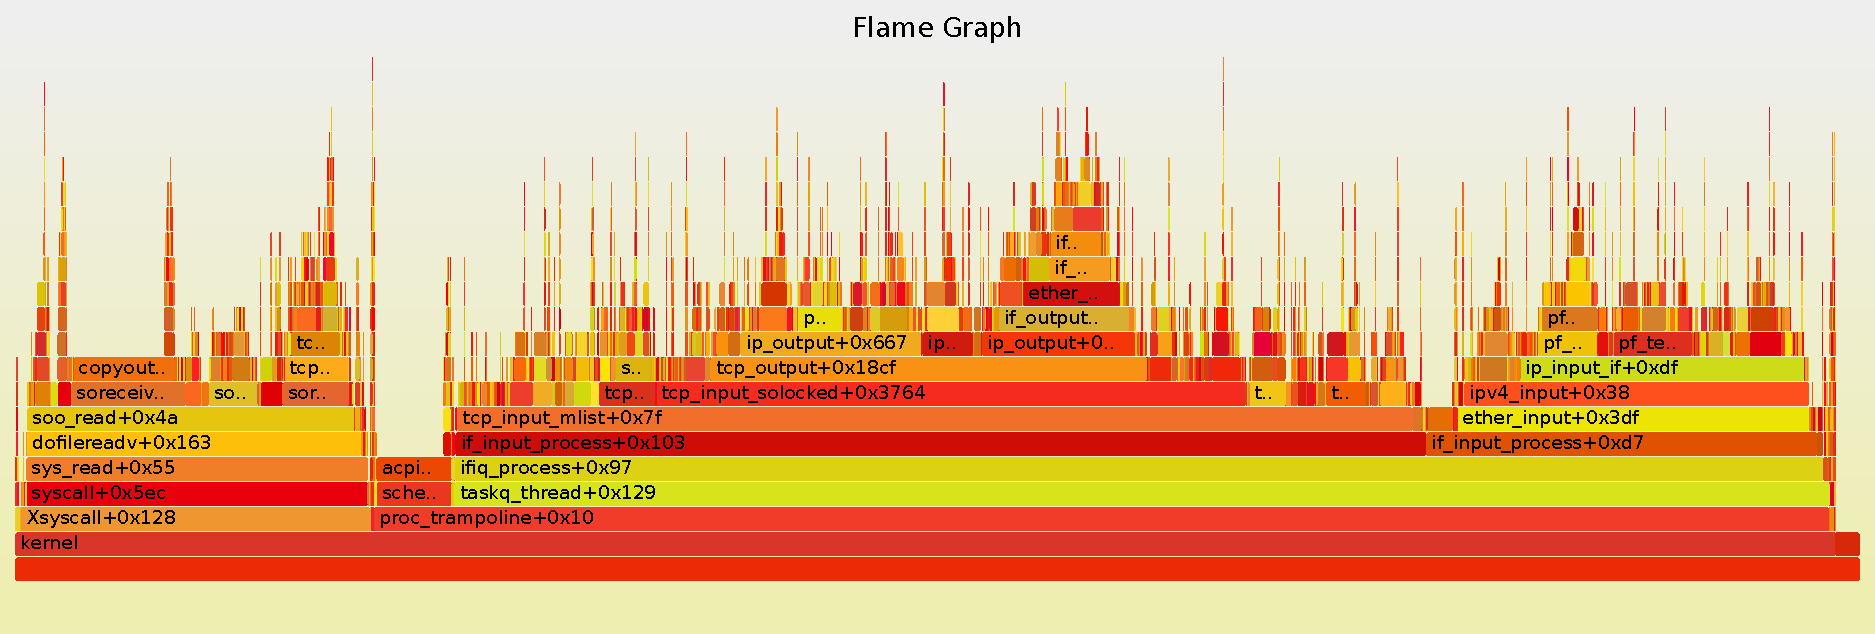
\includegraphics[width=\textwidth]{kstack/sys-tcp-input-parallel-rev-parallel.pdf}
\end{frame}

\section{Speed}

\subsection{New 100 Gbit/sec Hardare}
\begin{frame}{New 100 Gbit/sec Hardare, from 2024}
    \includegraphics[height=0.8\textheight]{images/obsdlab-netlink-ot41.pdf}
\end{frame}

\subsection{Daily Results}
\begin{frame}{Daily Results}
    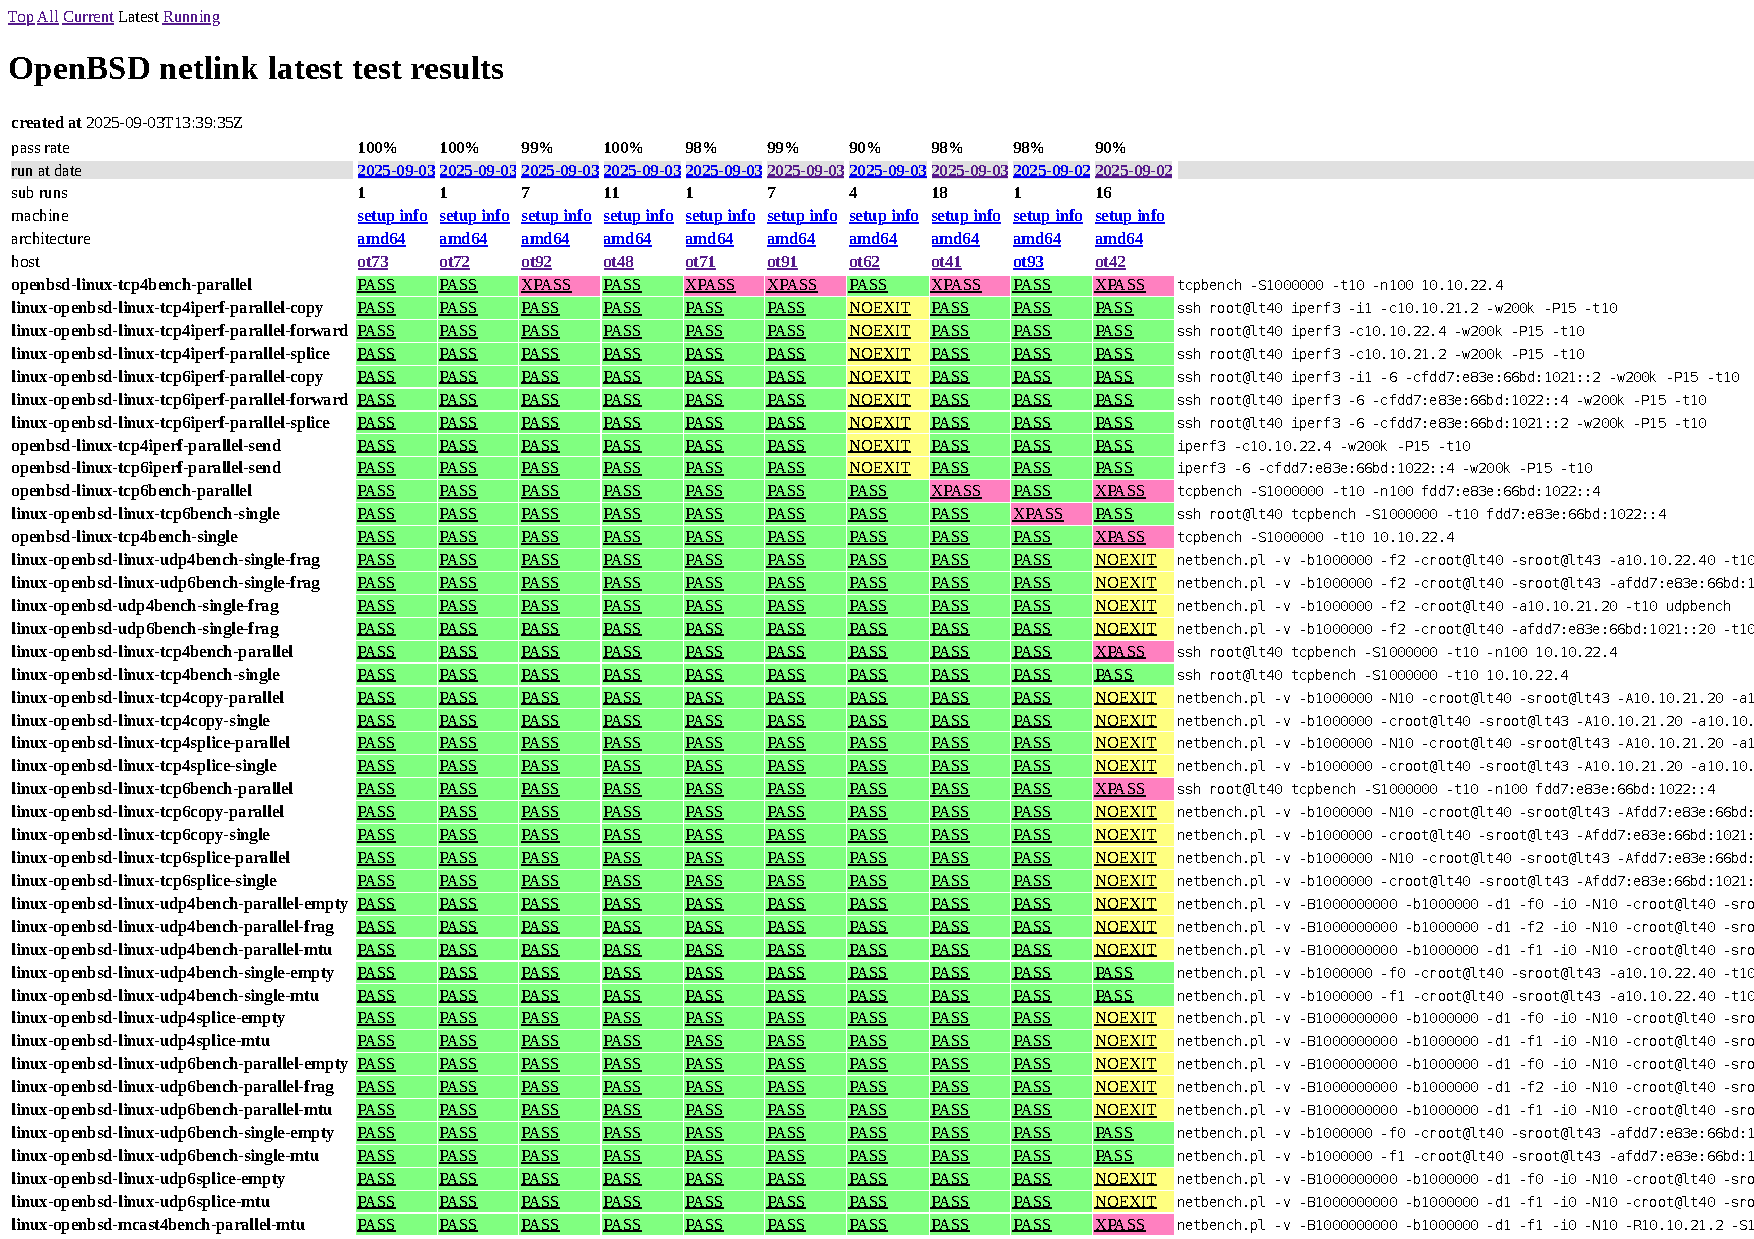
\includegraphics[height=0.8\textheight]{images/netlink-latest-chrome.pdf}
\end{frame}

\subsection{Test Matrix}
\begin{frame}{Test Matrix}
\begin{itemize}
    \item network hardware and driver\\
	bge bnxt em ice igc ix ixl re vio (vmx)
    \item modify network setup\\
	jumbo nolro nopf notso
    \item stack pseudo devices\\
	bridge carp gif gif6 gre veb vlan vxlan wg
    \item 93 test cases\\
	icmp tcp udp splice mcast iperf (trex)
    \item various platforms\\
	Intel AMD vmm-vmd KVM-qemu AMD-SEV (sparc64) (vmware)
\end{itemize}
\end{frame}

\subsection{Interface Throughput}
\begin{frame}{Daily Results}
    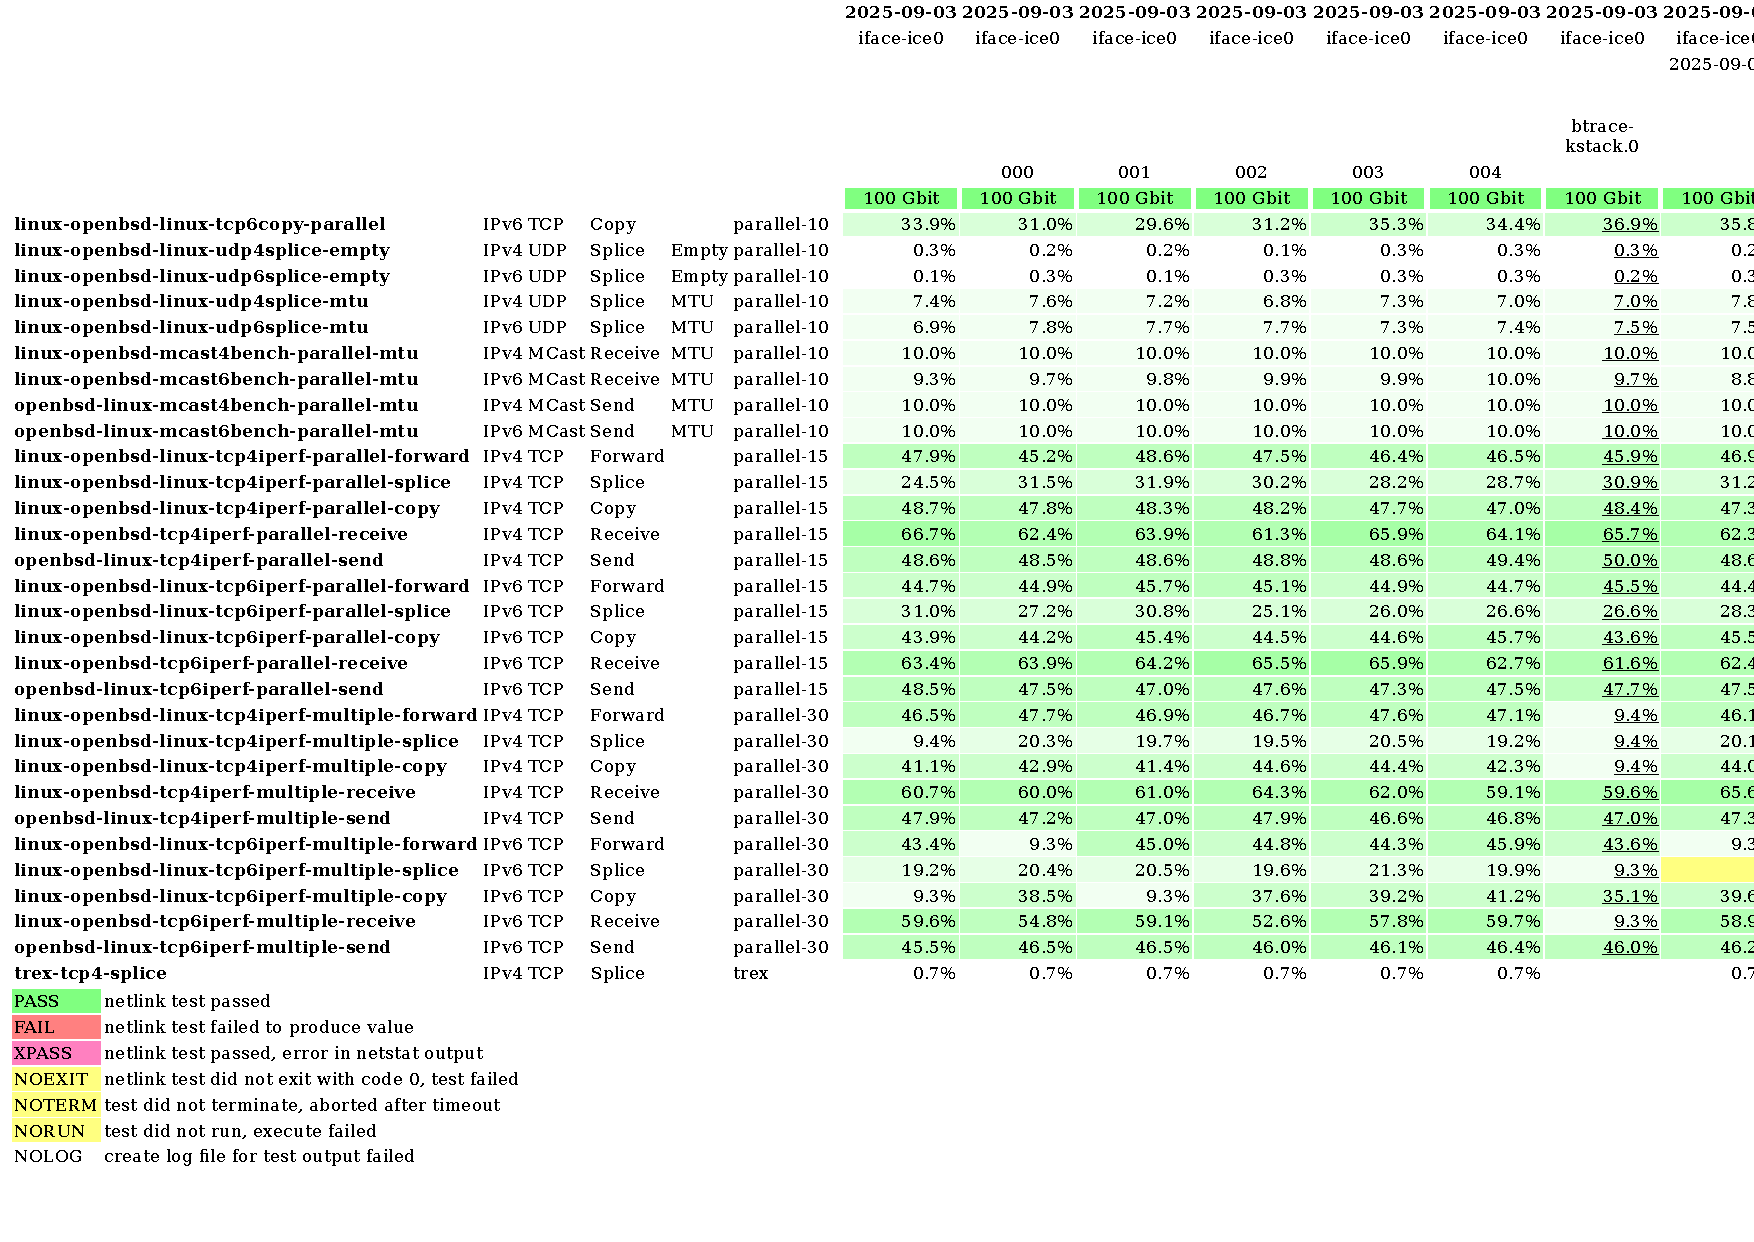
\includegraphics[height=0.8\textheight]{images/netlink-ice-firefox.pdf}
\end{frame}

\end{document}
